\newcommand{\co}{CO$^+$ }
\newcommand{\con}{CO$^+$}

\section*{Abstract}
We discuss newly measured rotational transitions of \co ($X ^2\Sigma ^+$) in its vibrational ground state $v=0$, in particular the fine-structure components of the $N=0-1$ and $N=1-2$ transitions. We employed a rotational action spectroscopic technique in a cryogenic ion trap for the measurements. The recorded low-temperature and high-resolution spectra of \co show resolved Zeeman splittings caused by the Earth’s magnetic field. The highly accurate experimental transition frequencies and derived molecular constants agree with previous measurements and improve the spectroscopic parameters for this known interstellar molecular ion.
\clearpage

\section{Introduction}

Carbon monoxide, CO, is the second most abundant molecule  in the interstellar medium (after H$_2$). In its ionic form, \con, it was first detected in interstellar photo-dissociation regions (PDRs) and planetary nebulae (PNs) by \citet{Latter1993}.  Later studies  confirmed the presence of \co  in several other dense PDRs, PNs and reflection nebulae \cite{Stoerzer1995, Fuente1997, Fuente2003, TFS2016, GCP2017}, and also in an external galaxy \cite{Fuente2006}. A search for \co in the diffuse interstellar medium has been unsuccessful so far, but the obtained upper limits on its abundance provide crucial information on the origin of CO in these regions \cite{GL2021}.\\

The rotational spectrum of the \co (X$^2\Sigma ^+$, $v$=0) molecular ion has been rather extensively studied previously. The pure rotational spectrum of its two lowest fine-structure components $N=0-1$ was first measured by \citet{Dixon1975} by a direct absorption experiment through a CO discharge. The spectral coverage was later extended to higher frequencies by \citet{Sastry1981} covering the $N=1-2$ through $N=3-4$ transitions, and  \citet{heuvel_dymanus_1982} measured the first far-infrared (supra THz) $N=8-9$ transition of \con. A recent study from \citet{Spezzano2013} extended the range up to 1.3 THz (up to $N=10-11$) and also provides the to date most accurate spectroscopic parameters for \co and its isotopologues based on an isotopically invariant fit. \\


Interestingly, so far the astronomically observed \co emission lines indicate that the rotational excitation temperatures are typically around 10~K \cite{Latter1993}, which is much lower than the surrounding PDR. This anomaly is yet to be clearly understood; \citet{Stauber2009} suggested this may be due to \co being excited upon formation. On the other hand, this suggests the need of  accurate laboratory measurements at low temperatures for astronomical detections of molecular ions. \\

The previous laboratory measurements of the \co molecular ion as discussed above were based on direct absorption experiments through liquid-nitrogen cooled DC glow discharges. This approach poses some challenging limitations for achieving very high spectral resolution, mainly due to the high kinetic and excitation temperatures in the discharge, leading to large Doppler linewidths and partition functions, and due to difficulties in producing the reactive ions with sufficient number density, leading to low signal-to-noise spectra. Another complication arises from background contamination from other species that are formed in the discharge. These limitations can be avoided by employing action spectroscopic methods based on sensitive  mass-spectrometric techniques, which measure the change in chemical composition of ions when they interact with resonant radiation light. This can offer several advantages such as mass selection and storage in a cold ion-trap, which leads to uncontaminated spectra and narrow linewidths. The first realization of pure rotational action spectroscopy in a cryogenic trap was shown by Schlemmer and coworkers \cite{Asvany2008} using a direct rotational laser induced reaction (LIR) method. Further action spectroscopic techniques were later developed to generalise the scheme for a  wide range of molecular ions, such as rotation-vibration double resonance - via LIR \cite{Gartner2013,jusko_two-photon_2014}, via predissociation \cite{Topfer2018}, or via laser induced inhibition of complex growth (LIICG)  \cite{Markus2019}. Another direct method for high-resolution rotational action spectroscopy is rotational state-dependent attachment of rare gas atoms (ROSAA) \cite{brunken_laboratory_2014,Brunken2017}, which is used in the present study. A detailed review of these techniques was recently provided by Asvany and Schlemmer \cite{Asvany2021}. \\

In this study, we used the ROSAA action spectroscopic method \cite{Brunken2017} to record several low $N$ rotational transitions of \co in a 4K-cryogenic ion trap instrument. The open shell \co molecular ion in its ground electronic and vibrational state has $^2\Sigma ^+$ symmetry. Each rotational quantum state $N$ splits into two fine-structure components ($N_J=N \pm 1/2$) due to the presence of the uncoupled electron spin $S=1/2$. The allowed transitions are $\Delta N = 1$ and $\Delta J = 0, \pm 1$. In the presence of a magnetic field each $N_J$ levels splits further into $2J+1$ Zeeman components, thereby lifting the angular momentum degeneracy. In fact, the \co ground state $N=0-1$ rotational transition  was already targeted by us using this technique in an earlier study \cite{Brunken2017}. Interestingly, only the $\Delta J=1$, $N_J=0_{1/2}-1_{3/2}$ transition was observed at the time (without any observable sub-structure due to Zeeman splitting), with a signal strength ten times higher than the $3\sigma$ noise level at the position of the $\Delta J=0$,  $N_J=0_{1/2}-1_{1/2}$ transition. At the time it was speculated whether this non-detection is related to intrinsic quantum-mechanical state-dependent effects during the formation of the He-\co complex. This puzzling finding partly motivated the current study.
 In this work we present and discuss the measured high-resolution pure rotational transitions of \co ($X ^2\Sigma ^+, v=0$), namely the $N_J$=$0_{1/2}-1_{1/2}$, $0_{1/2}-1_{3/2}$, $1_{3/2}-2_{3/2}$ and $1_{1/2}-2_{3/2}$ transitions. We observe clearly resolved Zeeman splittings for the $0_{1/2}-1_{1/2}$ transition caused by the Earth’s magnetic field.

\section{Experiment}
\label{sec:method}

\begin{figure}[!htb]
     \centering
     \begin{subfigure}[b]{0.49\textwidth}
         \centering
         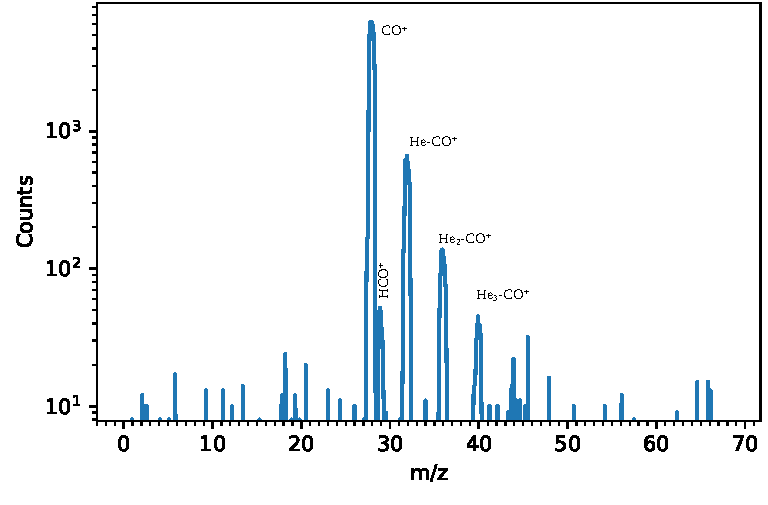
\includegraphics[width=1\textwidth]{chapters/CO+_ROSAA_paper/CO+_masspec.pdf}
         \caption{}
         \label{fig:CO+:masspec}
     \end{subfigure}
     \hfill
     \begin{subfigure}[b]{0.49\textwidth}
         \centering
         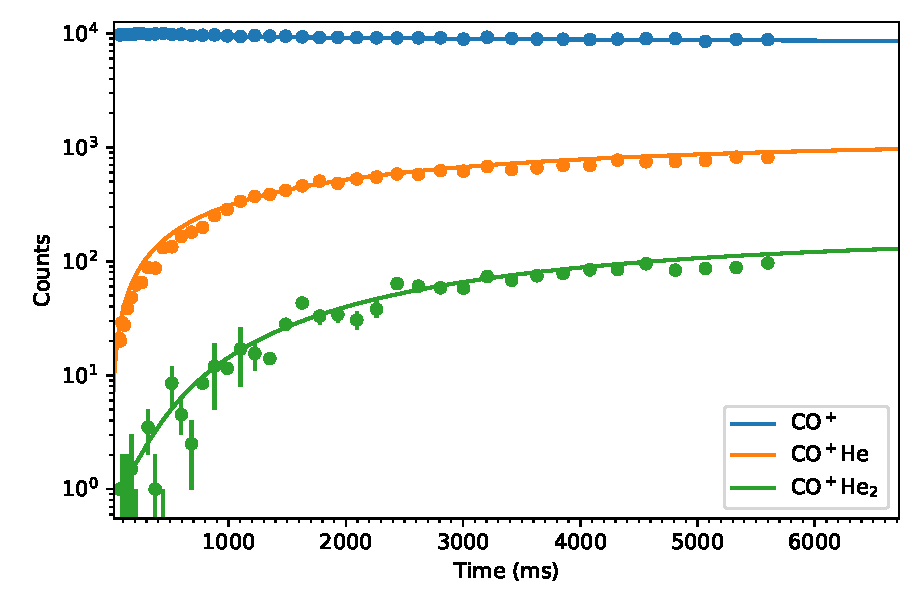
\includegraphics[width=1\textwidth]{chapters/CO+_ROSAA_paper/CO+_kinetics.pdf}
         \caption{}
         \label{fig:kinetics}
     \end{subfigure}
     
        \caption{(a): Measured mass spectrum after storing \co ions (m/z 28) for $\sim$600~ms in the cryogenic ion trap using He buffer gas ($\sim 4\cdot10^{14}$~cm$^{-3}$ number density, T=4.7(3)~K), showing the \co ion and the subsequent formation of ion-He complexes with up to three He atoms attached. A small contamination from HCO$^+$ can be seen, resulting from insufficient mass-filtering of the primary ions. (b): The counts of primary and complex ions are monitored as a function of trap time ($\sim 1.5\cdot10^{14}$~cm$^{-3}$, T=4.7(3)~K). The formation ($k_{3_1}$) and dissociation rate ($k_{CID_1}$) constants as described in Eq. \ref{eqn:fulleq} are derived by numerical fitting.}
        \label{fig:masspec-kinetics}
\end{figure}

The rotational spectra of \co  were recorded with a novel action spectroscopic scheme ROSAA using the FELion cryogenic 22-pole ion trap instrument. A detailed account of the FELion instrument is provided in Section \ref{sec:felion} and the ROSAA technique in Section \ref{sec:methods:rotation}. Here we only give a brief account of details specific to the \co ion. \\

The ions were produced by electron impact ionization (EI, electron energy 25~eV) from neutral CO precursor. A short pulse ($\sim$50~ms) of mass-selected (using quadrupole mass filter) \co is injected into the trap and stored for a specified time, typically $\sim$600~ms for spectroscopic experiments, with continuous inflow of He buffer gas for collisional cooling and complex formation. At low temperature (around $\sim 4.7(3)$~K ambient temperature in the present experiments) and high number density $\sim10^{14}$~cm$^{-3}$ of gas inflow, helium gas will readily attach to \co by ternary association and can dissociate by collision induced dissociation (CID): 

%\begin{equation}
%\text{CO$^+$ + 2He }
%\substack{\overset{k_{3_1}} \longrightarrow \\ \underset{k_{CID_1}} \longleftarrow}
%\text{He-CO$^+$  + He}
%\label{eqn:reaction}
%\end{equation}

\begin{equation}
\text{He$_{n-1}$-CO$^+$ + 2He}
\substack{\overset{k_{3_n}} \longrightarrow \\ \underset{k_{CID_n}} \longleftarrow}
\text{He$_n$-CO$^+$ + He }
\text{ ; where $n\geq 1$}
\label{eqn:fulleq}
\end{equation}

The efficient formation of complexes can be clearly seen in the mass spectrum shown in Figure \ref{fig:CO+:masspec}. The formed complex is mass filtered with a second quadruple mass-filter and detected with a single ion counting Daly detector\cite{daly_scintillation_1960}. \\

By measuring the primary \co and He-\co complex ion counts as a function of trap time, we measured the ternary association and collision induced dissociation rate coefficients as shown in Figure \ref{fig:kinetics}. At a nominal trap temperature of  $\sim 4.7(3)$~K, translating to a collisional temperature of $ \sim 6$~K caused by the higher kinetic energy ($\sim 15$~K) of the ions in the radio-frequency trap, we obtained $k_{3_1}=1.74(1)\cdot10^{-30}$ cm$^6$s$^{-1}$, and  $k_{CID_1}=2.01(4)\cdot10^{-15}$ cm$^3$s$^{-1}$ .\\

\begin{figure}[!htb]
    \centering
    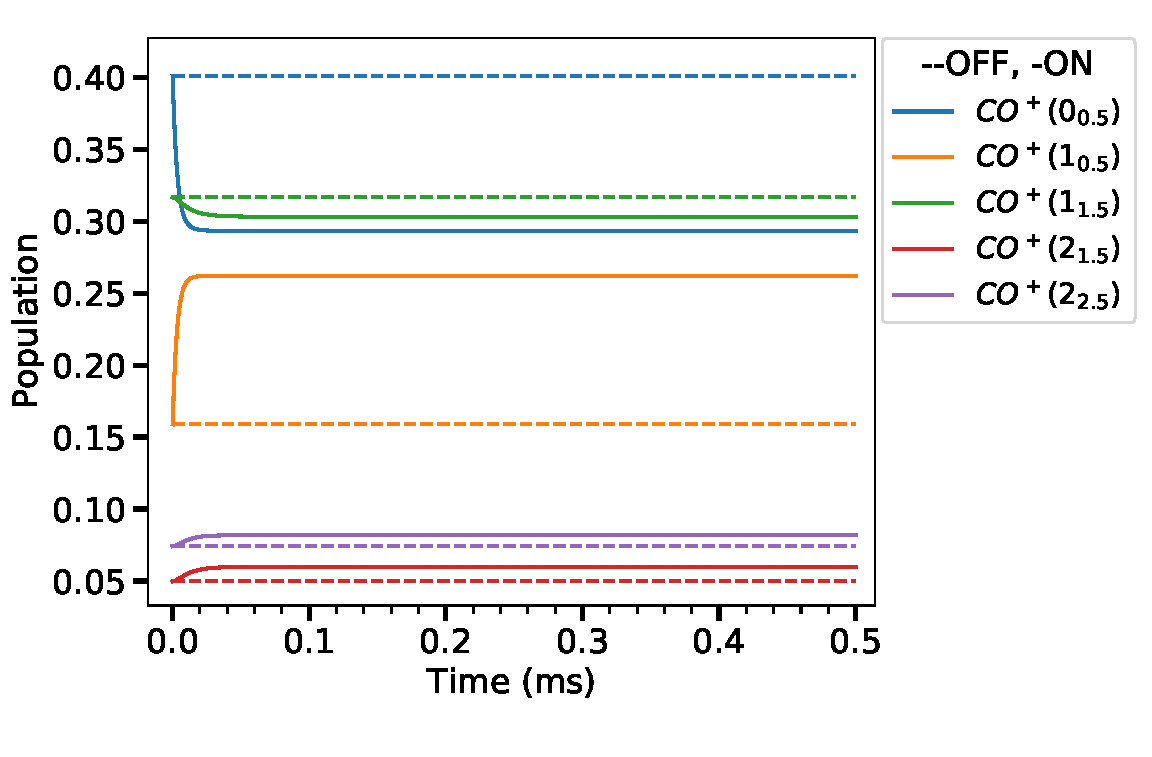
\includegraphics[scale=0.4]{chapters/CO+_ROSAA_paper/CO+_population.pdf}
    \caption{\co ($X ^2\Sigma ^+, v=0$): Numerical simulation of rotational population distribution of $N_J$ states with (-ON) and without (--OFF) radiation for the $N_J=0_{1/2}-1_{1/2}$ transition. At t=0, the initial population is given by a Boltzmann distribution (at collisional temperature T=$6(1)$ K) and the collisional rates (with He number density [He]=$4\cdot10^{14}$~cm$^{-3}$) are derived from He-\co collisional rate constants values \cite{CO+He_collision}. The radiation rates (Einstein B  coefficients for stimulated emission and absorption) are derived from Einstein A coefficients for  spontaneous emission (PGOPHER simulation \cite{western_pgopher_2017}). }
    \label{fig:population}
\end{figure}

    \begin{figure}
        \centering
        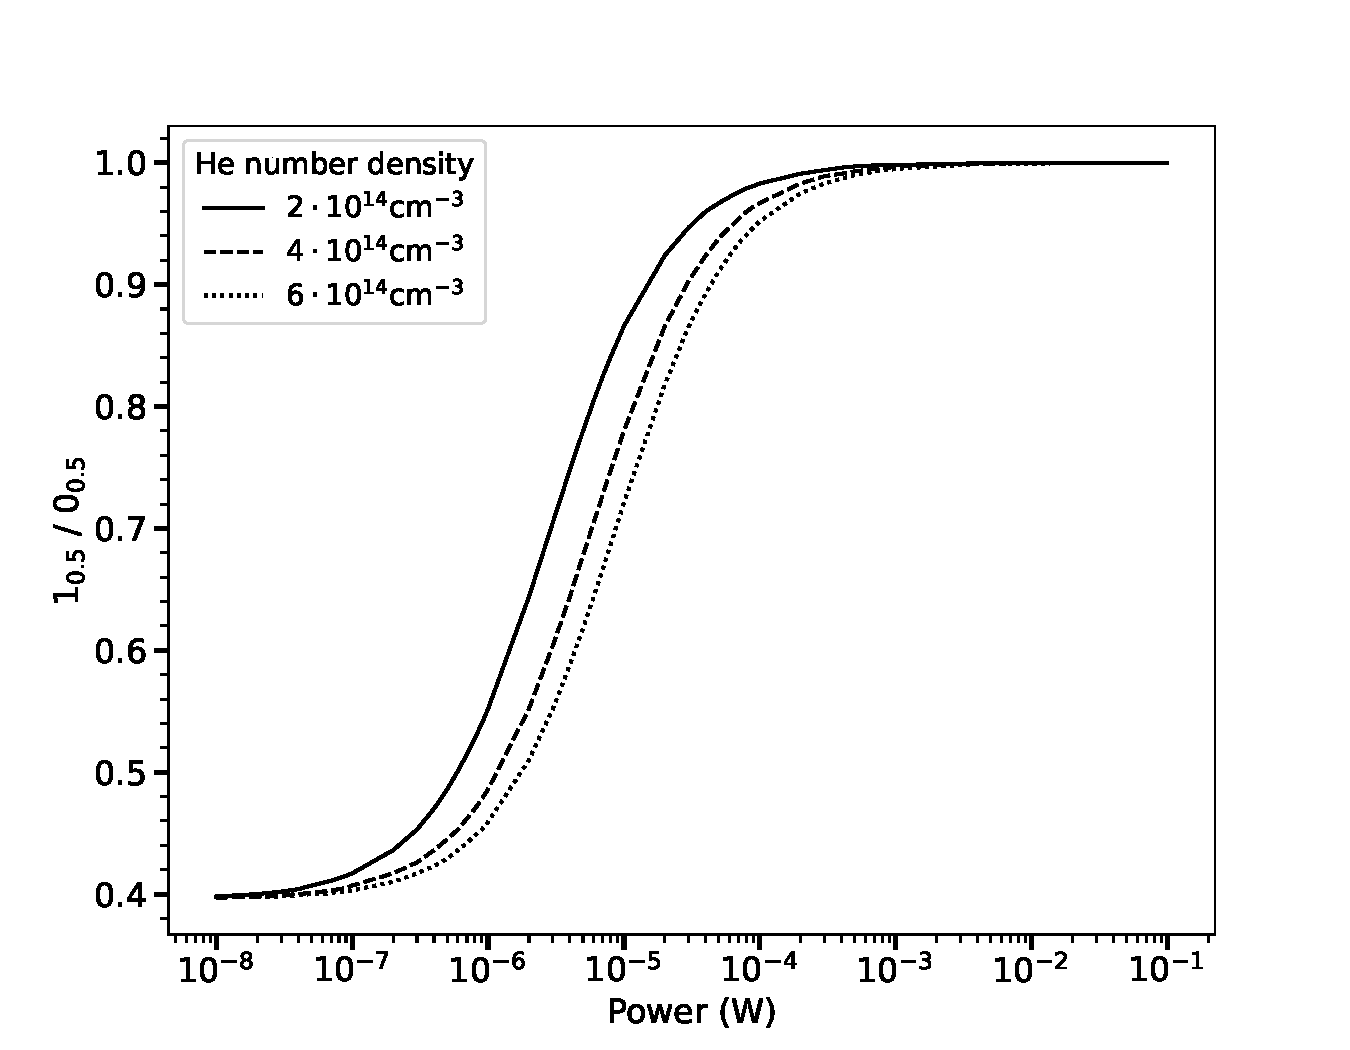
\includegraphics[scale=0.4]{chapters/CO+_ROSAA_paper/comapreNumberDensity.pdf}
        \caption{Simulated population ratio ($N_J$: up/down) of the CO$^+$ $N_J=0_{1/2}-1_{1/2}$ transition as a function of excitation power, at different He number densities, after storing for 600~ms in the trap. Lower He number densities lead to saturation of the transition at lower excitation power.}
        \label{fig::power-dep}
    \end{figure}

For measuring rotational transitions of \co we employed the ROSAA technique, which utilises the change in the helium attachment rate to molecular ions depending on their internal excitation, i.e, ions with certain  quantum number $N_J$ have different attachment rate coefficients for forming He-\co clusters with Helium. The measured $k_3$ rate coefficient given above is actually a  weighted averaged rate coefficient over the thermal population of rotational levels, i.e., the Boltzmann distribution close to the nominal trap temperature, reached by He collisions with a rate of $\sim 10^4$~s$^{-1}$ at the typical number densities used in the experiments. Upon resonant excitation the thermal equilibrium distribution is disturbed by competing radiative processes (typically with comparable rates of $\sim 10^5$~s$^{-1}$ for the \co ground state transitions), leading to a change in the attachment rate and thus number of formed complexes. Hence, the measured signal intensity ($S$) is given as the observed change (in \%) of the number of He-\co complexes formed between the set frequency ($I_{ON}$) and a fixed reference frequency ($I_{OFF}$, offset about 3~GHz from scanning range), and scaled by $I_{OFF}$, i.e, $ S=(I_{OFF} - I_{ON})/I_{OFF} $, after storing for a fixed time of 600~ms in the trap at each data point. The spectra are measured in 10~kHz steps and are averaged over 70 iterations. \\

The temporal changes in rotational level population, neglecting Zeeman splitting, without and with radiation (switched on at $t=0$) are shown exemplary for excitation of the $N"_{J"}-N'_{J'}$=$0_{1/2}-1_{1/2}$ transition and typical experimental conditions (radiation power $\sim 25\,\mu$W, He number density $4\cdot 10^{14}$~cm$^{-3}$) in Figure \ref{fig:population}. We used collisional rate coefficients for the He-\co system that were recently calculated \cite{CO+He_collision} and Einstein coefficients determined using the PGopher program suite \cite{western_pgopher_2017}.
The dependence of the ratio of the upper-to-lower level population  $N'_{J'}/N"_{J"}=1_{1/2}/0_{1/2}$ on the radiation power in the trap at different He number densities is shown in Figure \ref{fig::power-dep}. The actual power of 25~$\mu$W used in the experiments to minimize power broadening is only slightly below the saturation power for the used He number density of $4\cdot 10^{14}$~cm$^{-3}$. Without radiation the ratio is $0.4$, with a total population of $P_{tot}=(16+40)\%=56$~\% in both states, given by the Boltzmann distribution. The maximum achievable population change upon radiation leads to a ratio corresponding to the statistical weight ratio of $(2J'+1)/(2J"+1)=1$, with the same total population of 56~\% in both states, i.e., the percentage of molecular ions addressed directly by the applied radiation. An upper limit on the observable depletion signal can be estimated by, albeit unrealistically, assuming that all states except the excited one form complexes with the same rate, and the excited one does not form complexes at all: $S_{max}\approx 14$~\%. In reality the depletion signal will be lower depending on the actual change in the attachment rate coefficient for different rotational levels, and by the Zeeman splitting of the lower state levels, leading to an equal partitioning of the overall population over the two Zeeman states. Numerical simulations for other rotational transitions are shown in the Supplementary Information.\\

As radiation source we used a continuous wave Signal Generator Extension (SGX) Module (VDI - Virginia Diode, Inc. WR9.0-SGX) to cover the $N_J$=$0_{1/2}-1_{1/2}$, $0_{1/2}-1_{3/2}$ transitions at frequencies around 117 and 118~GHz, respectively. For the  $N_J$=$1_{1/2}-2_{3/2}$ and $1_{3/2}-2_{3/2}$ transitions we used an additional frequency doubler (WR9.0SGX + WR4.3X2) to reach approximately 235~GHz. The SGX is driven by a  muwave signal generator (R\&S \textsuperscript{\textregistered} SMB100A) disciplined by an atomic clock (Stanford Research Systems - FS740). Intrinsic radiation linewidths are better than 1~kHz and the relative frequency accuracy is specified to be better than $1\cdot 10^{-13}$. The radiation is directed into the trap through a 0.6~mm thick CVD diamond window (Diamond Materials GmbH) with a conical horn antenna. The maximum output power of this radiation source setup is $\sim$20~mW ($\sim$3~mW when using the doubler), which can be regulated. Considering the geometrical aspect and distance of the trap from the source, around $\sim 5$~\% of the output is reaching the trap center. We did not attempt to compensate for the Earth magnetic field, as was done in earlier absorption measurements \cite{Bogey1982}.

\section{Results and discussions}

\begin{figure}[!htb]
    \centering
    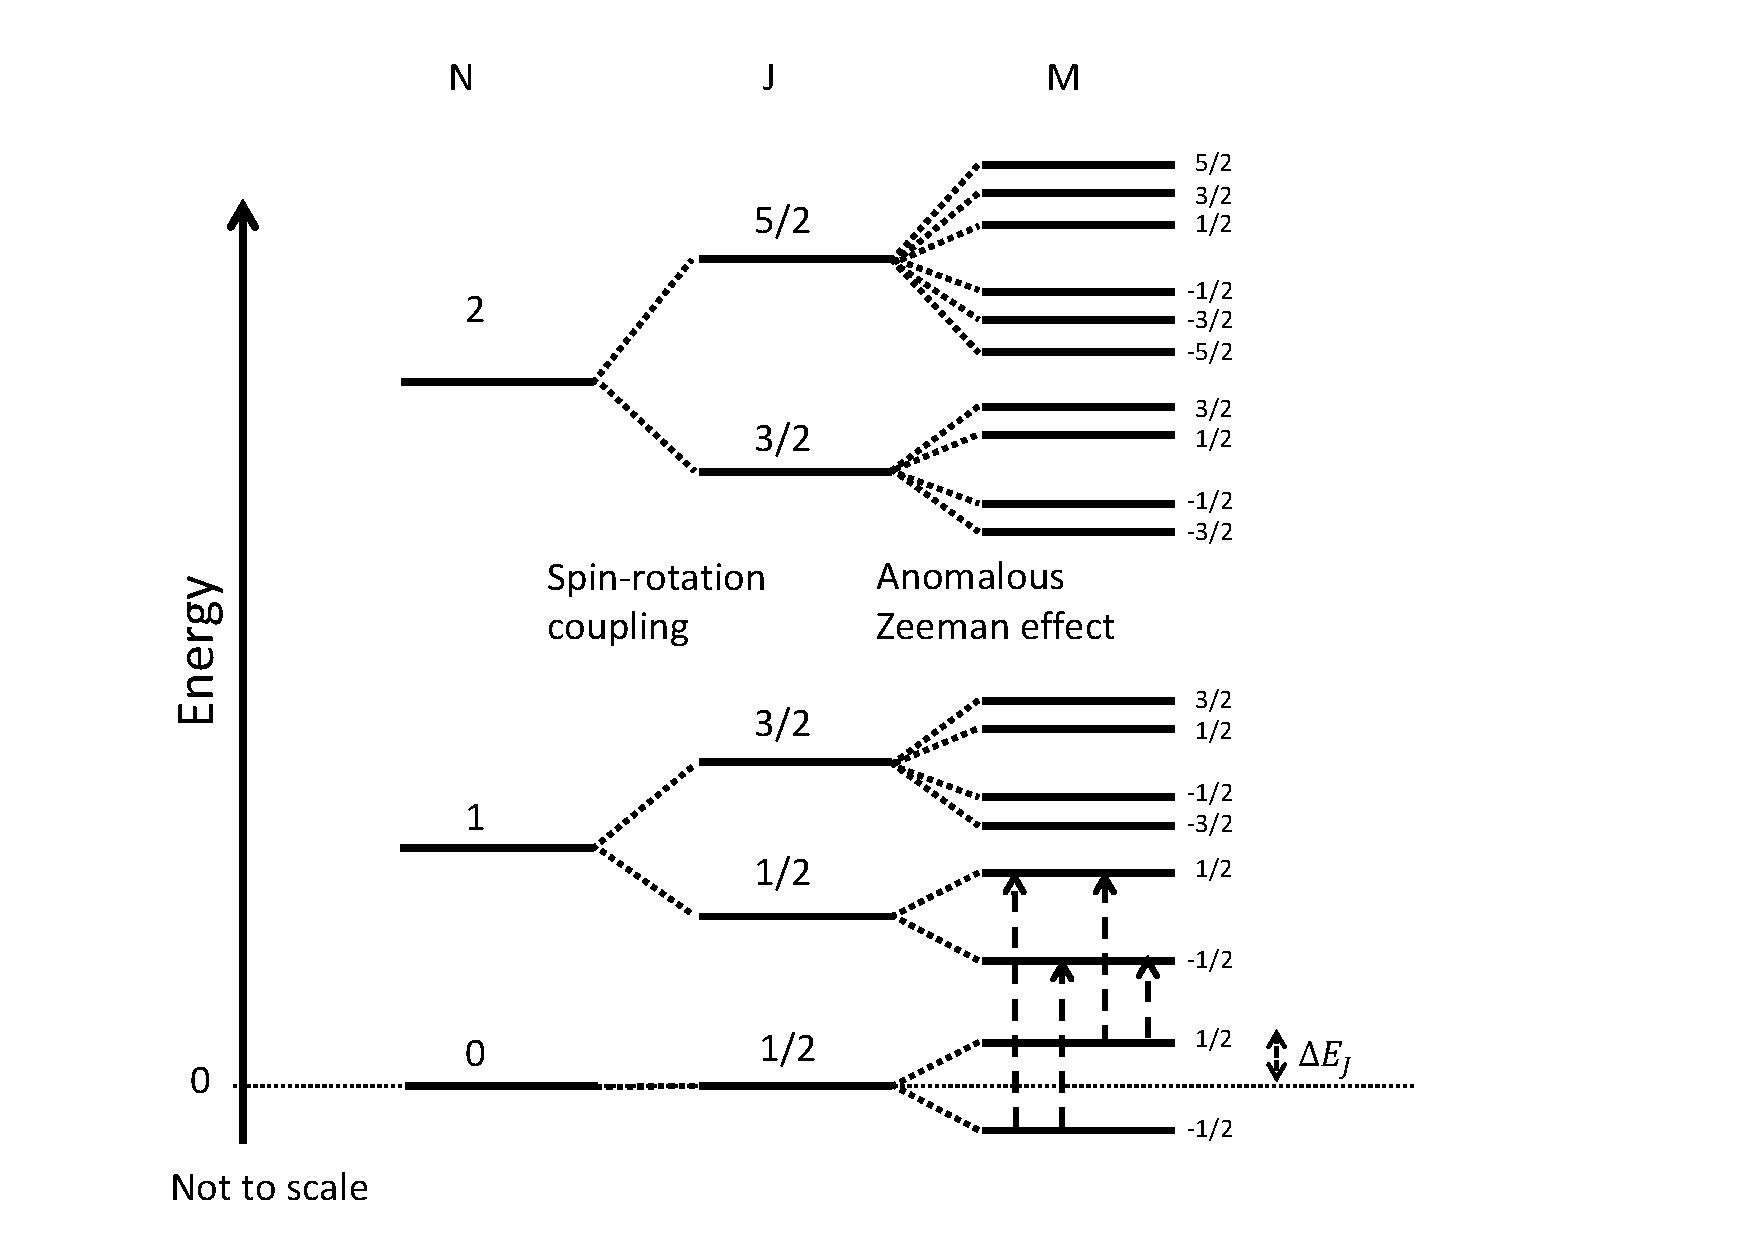
\includegraphics[scale=0.4]{chapters/CO+_ROSAA_paper/CO+_energy_levels.pdf}
    \caption{Rotational energy level diagram for \co ($X$ $^2\Sigma ^+, v=0$) showing fine-structure and Zeeman splittings (not to scale). The dashed arrow lines show the expected Zeeman components of the $N_J=0_{1/2}-1_{1/2}$ transition. $\Delta E_J$, the magnetic interaction energy is given by Equation \ref{eqn:zeeman}.}
    \label{fig:energy}
\end{figure}

\begin{figure}[!htb]
    \centering
    \begin{subfigure}[b]{0.49\textwidth}
        \centering
        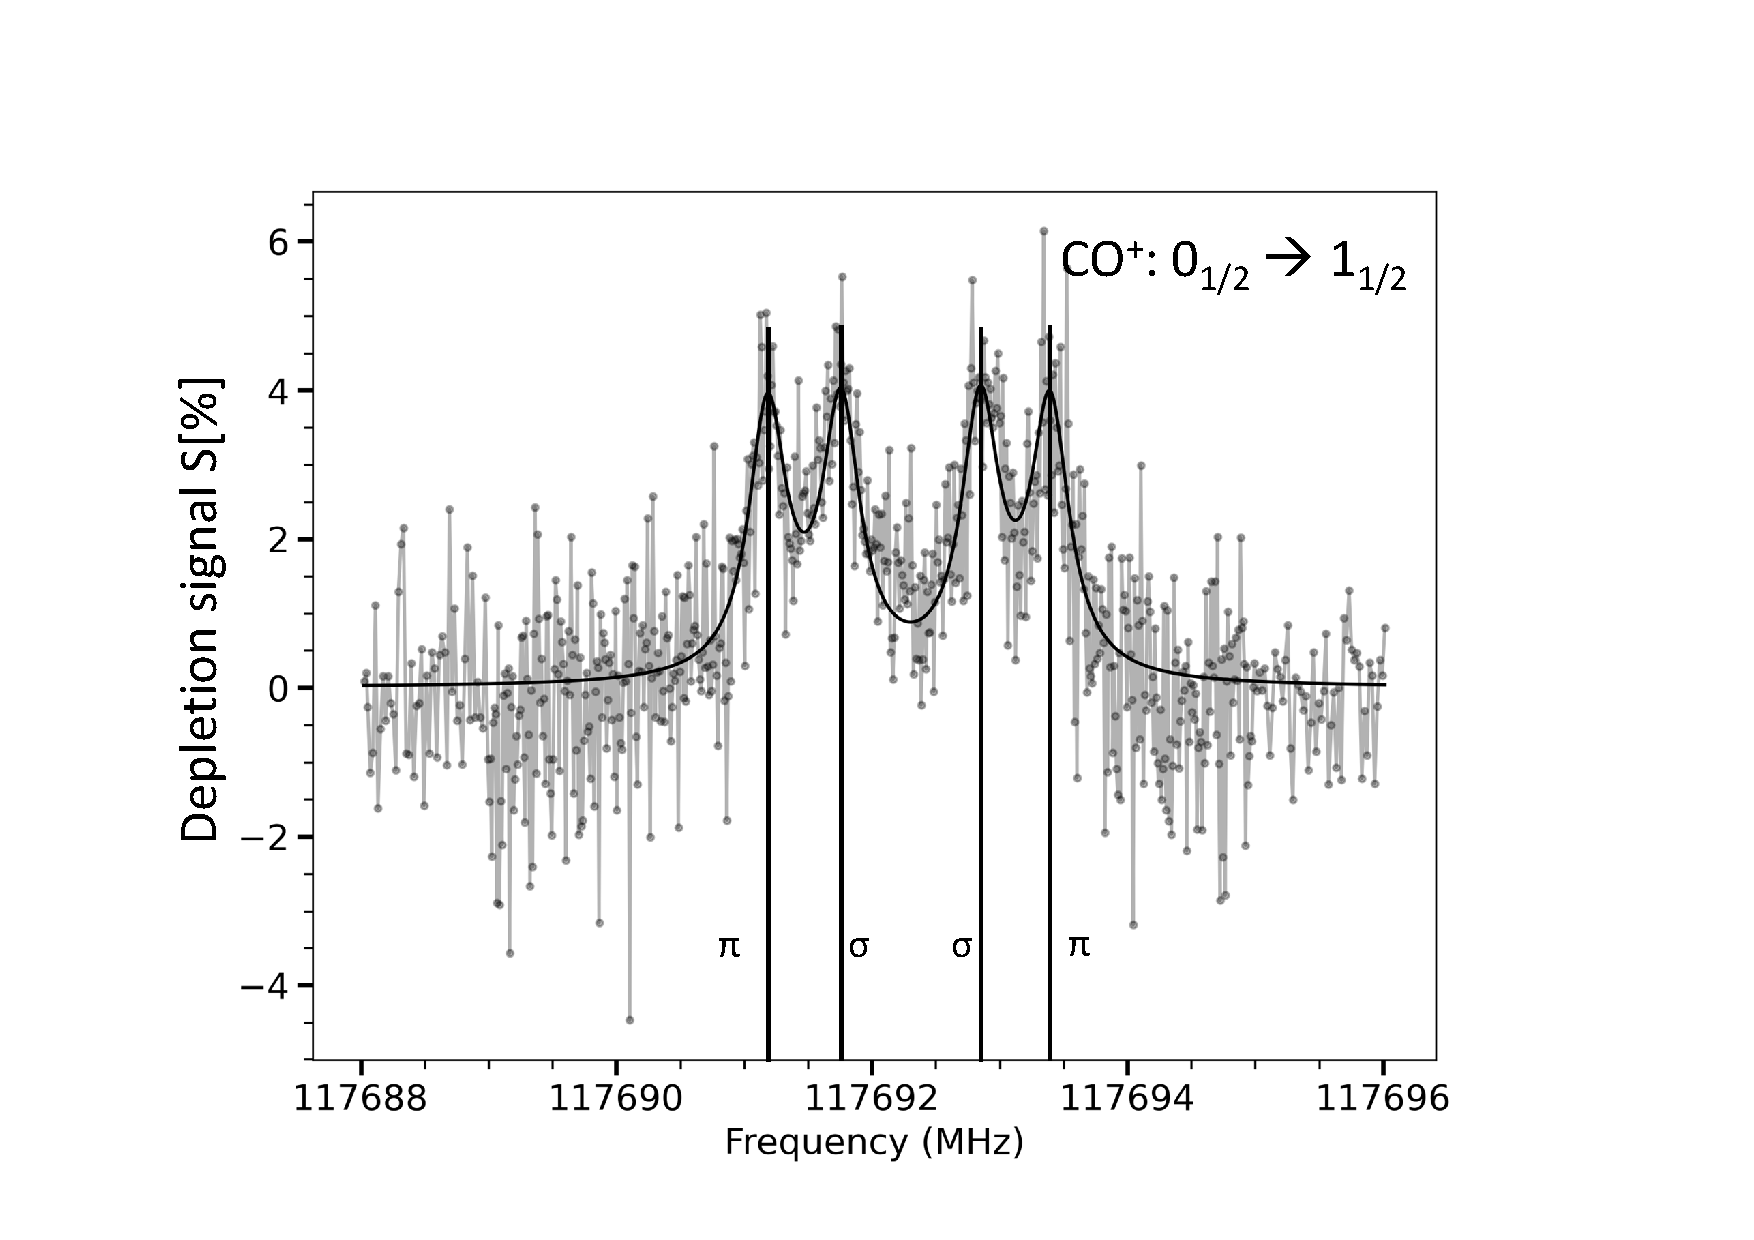
\includegraphics[width=1\textwidth]{chapters/CO+_ROSAA_paper/117_CO+_fig.pdf}
        \caption{}
        \label{fig:117}
    \end{subfigure}
    \hfill
    \begin{subfigure}[b]{0.49\textwidth}
        \centering
        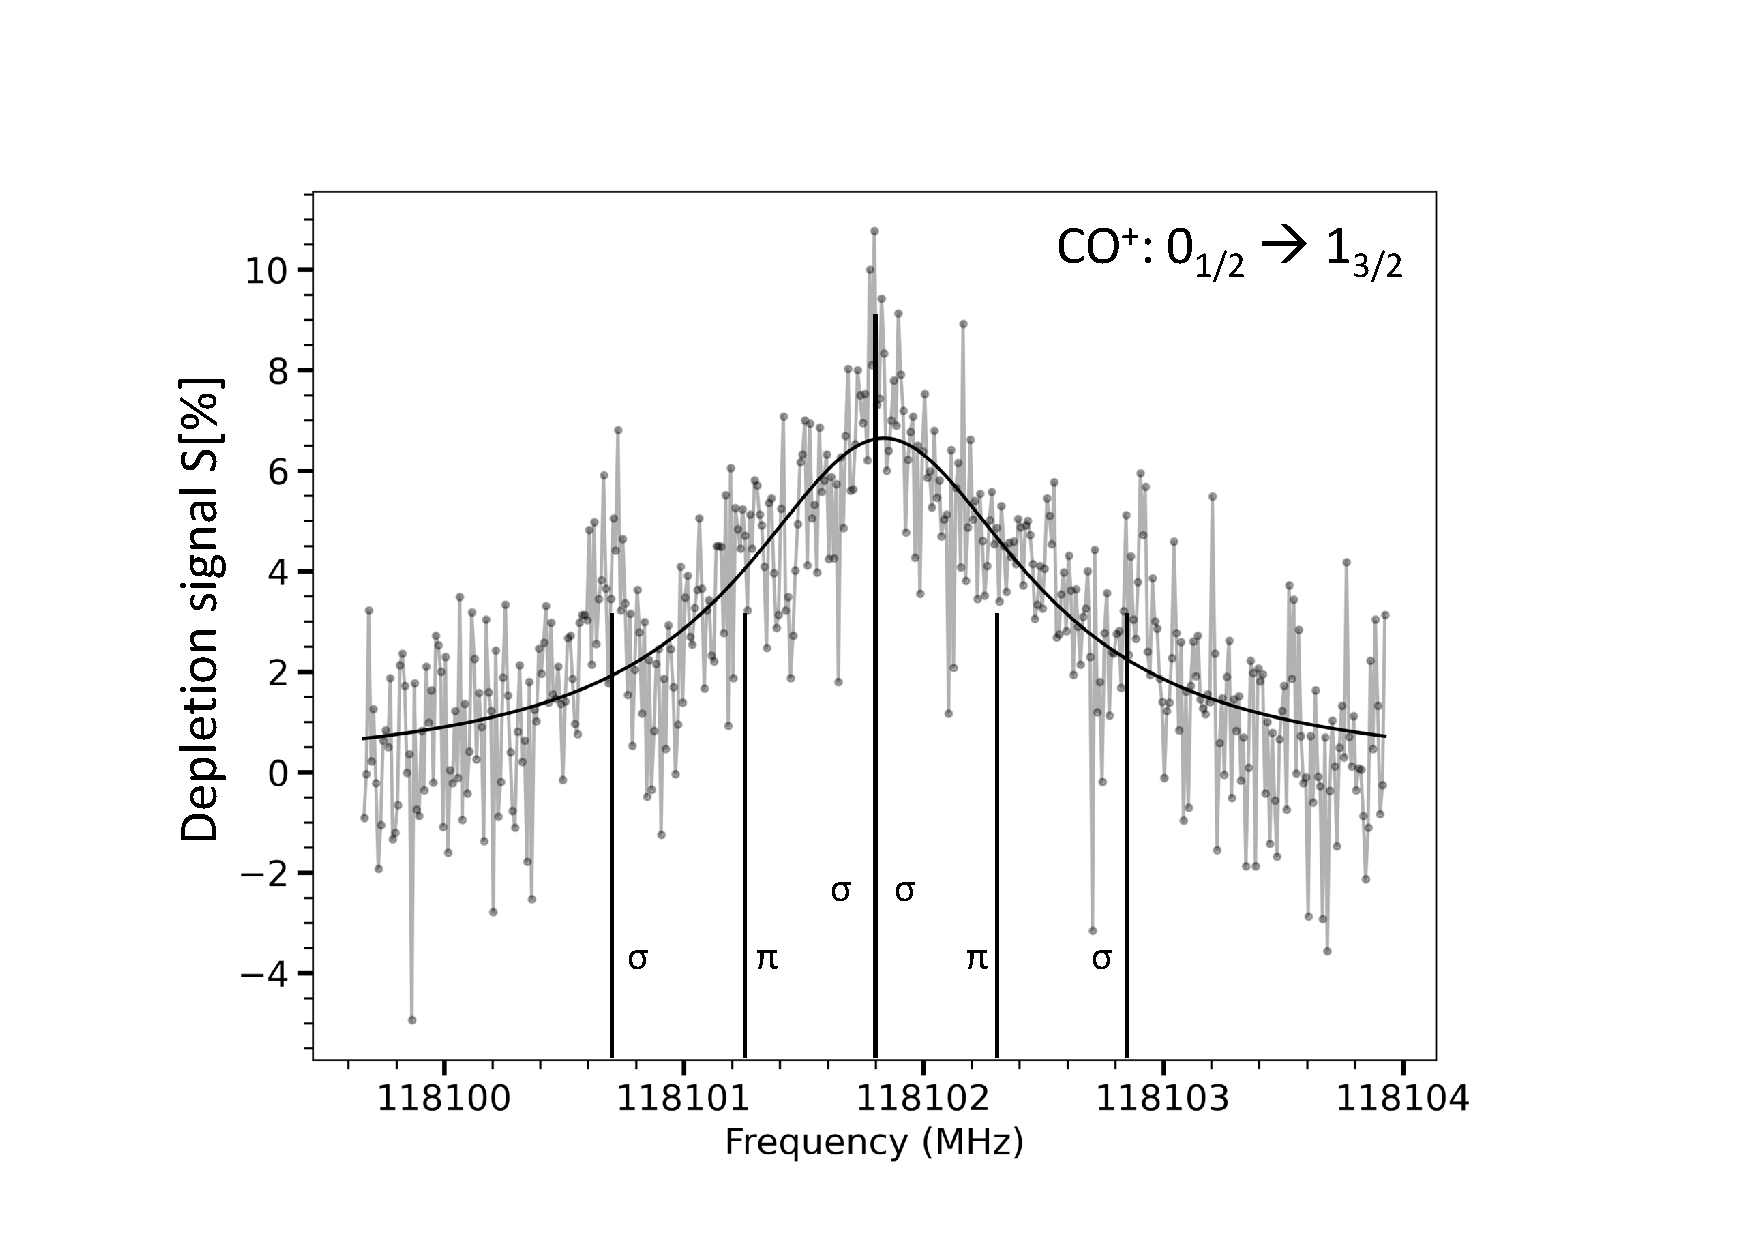
\includegraphics[width=1\textwidth]{chapters/CO+_ROSAA_paper/118_CO+_fig.pdf}
        \caption{}
        \label{fig:118}
    \end{subfigure}
    \hfill
    \begin{subfigure}[b]{0.49\textwidth}
        \centering
        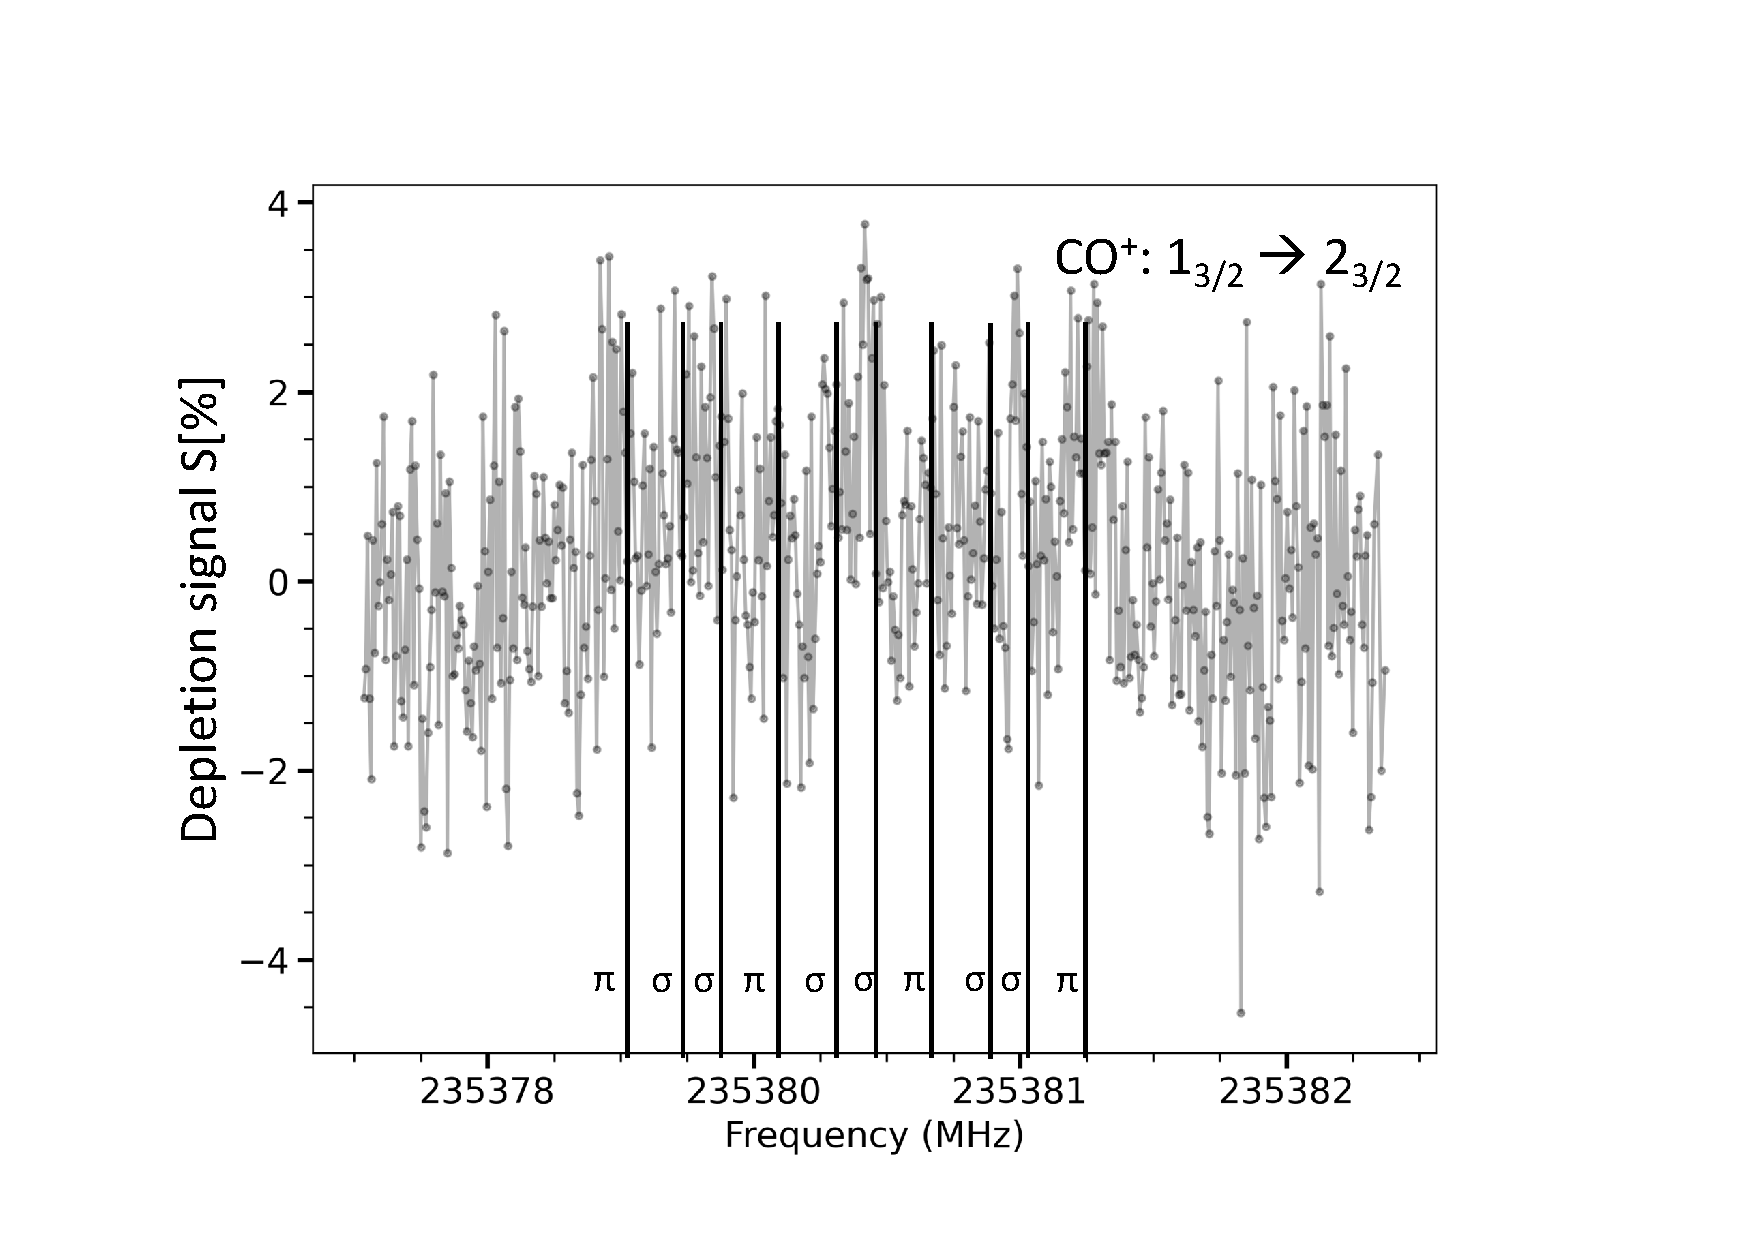
\includegraphics[width=1\textwidth]{chapters/CO+_ROSAA_paper/235_380_CO+_fig.pdf}
        \caption{}
        \label{fig:235_380}
    \end{subfigure}
    \hfill
    \begin{subfigure}[b]{0.49\textwidth}
        \centering
        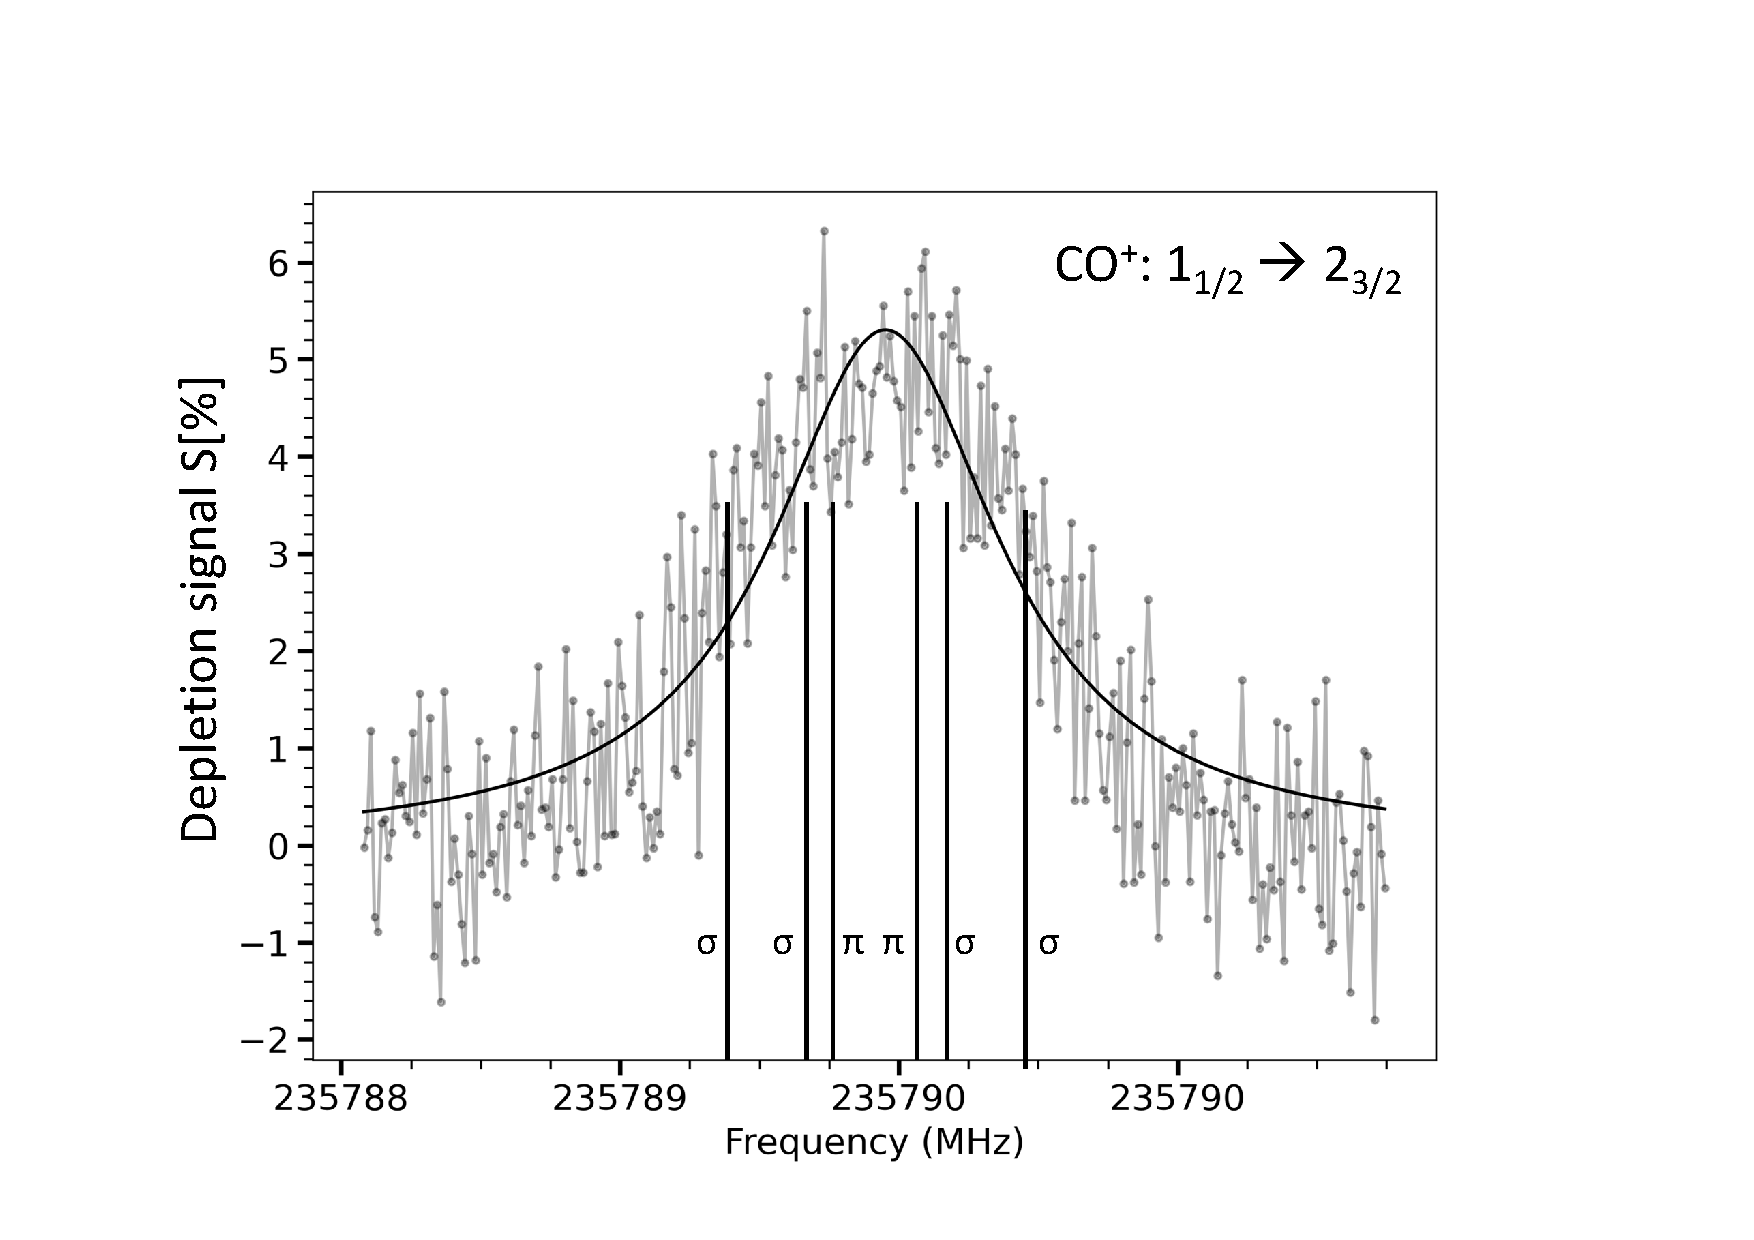
\includegraphics[width=1\textwidth]{chapters/CO+_ROSAA_paper/235_789_CO+_fig.pdf}
        \caption{}
        \label{fig:235_789}
    \end{subfigure}
    \caption{Measured rotational transitions of the \co molecular ion in the presence of Earth magnetic field causing anomalous Zeeman splitting. The $\sigma$ and $\pi$ correspond to perpendicular ($\Delta M=\pm1$) and parallel ($\Delta M=0$) magnetic field, respectively, w.r.t electric field.}
    \label{fig:full}
\end{figure}

We targeted four fine-structure lines of \con, of which three were detected as shown in Figure \ref{fig:full}. The signal-to-noise ratio of the $1_{3/2}-2_{3/2}$ transition is very low, thus no transition frequencies were extracted in this case. As shown in Figure \ref{fig:energy}, each $N_J$ levels splits further into $2J+1$ Zeeman components in the presence of a magnetic field. The splitting energy, i.e, magnetic interaction energy ($\Delta E_J$) of each $N_J$ state at low magnetic-field strengths is defined as:
\begin{equation}
    \text{$\Delta E_J = g_J \cdot M_J \cdot \mu _B \cdot B$}
    \label{eqn:zeeman}
\end{equation}

\noindent where
\begin{equation}
    g_J = g_S \cdot \frac{S(S+1)+J(J+1)-N(N+1)}{2J(J+1)}
    \label{eqn:gfactor}
\end{equation}

is the effective Landé g-factor \cite{Lande1921} for the Zeeman effect due to a weak magnetic field in the presence of net non-zero electron spin, $g_S=2.002318$ is the electron spin g-factor, $M_J$ is the magnetic quantum number, and $\mu_B$ and $h$ are Bohr magneton and Planck's constants, respectively. $B$ corresponds to the magnetic field strength, which can be derived from a fit to an effective Hamiltonian using PGOPHER \cite{western_pgopher_2017}. The allowed transitions follow $\Delta N=1=\pm 1$, $\Delta J = (0, \pm 1)$ and $\Delta M = (0, \pm 1)$. From our measurements we determined the total magnetic field as $B=\sim 60(1)\,\mu$T, which closely corresponds to the total Earth magnetic field (EMF) of  $\sim 49\, \mu$T at the location Nijmegen (The Netherlands). The small difference of the measured $B$ field from EMF is likely due to the nearby magnetic bearings of a high vacuum pump. Further, as shown in Figure \ref{fig:117} a), we see both $\sigma$ ($\Delta M=\pm1$) and $\pi$ ($\Delta M=0$) transitions of comparable strength, which indicates that the magnetic field is oriented under nearly $45^{\circ}$ relative to our vertically polarised radiation. However, due to the action spectroscopic method used, we would expect the same depletion signal for each of the Zeeman components once we saturate the transition. \\

\begin{table}[!htb]
        \centering
        \caption{Resolved Zeeman splitting for $N_J=0_{1/2}-1_{1/2}$ transition}
        \begin{tabular}{rcrc}
            $M^{''}$ & $\xrightarrow{}$ & $M^{'}$ & Frequencies (MHz)\\
            \\ \hline \hline \\
            +1/2 & $\xrightarrow{}$ & +1/2 & 117691.183 (14) \\
            -1/2 & $\xrightarrow{}$ & +1/2 & 117691.759 (14) \\
            +1/2 & $\xrightarrow{}$ & -1/2 & 117692.849 (14) \\
            -1/2 & $\xrightarrow{}$ & -1/2 & 117693.395 (14) \\
            \hline\\
            
        \end{tabular}
        \label{tab:zeeman}
    \end{table}

\begin{table}[!htb]
    \centering
    \caption{Rotational transition frequencies of \co ($X^2\Sigma^+$)}
    
    \begin{tabular}{rclrcc}
        $N"_{J"}$ & $\xrightarrow{}$ & $N'_{J^{'}}$ & Frequencies (MHz) & $O-C$ (kHz) & Prev. work\\ 
        \\\hline \hline \\
        $0_{1/2}  $ & $\xrightarrow{}$ & $1_{1/2}$  $^\star$$^\star$     &  117692.296 (007)  $^\star$    &   2.5   & 117692.360(030) $^d$ \\
        $0_{1/2}  $ & $\xrightarrow{}$ & $1_{3/2}$       &  118101.835 (023)  $^\star$    & 29.3 & 118101.812(050) $^d$ \\
        $1_{3/2}  $ & $\xrightarrow{}$ & $2_{3/2}$       &  235380.046 (150) $^a$         & 2.6 & \\
        $1_{1/2}  $ & $\xrightarrow{}$ & $2_{3/2}$       &  235789.555 (011)  $^\star$    & -4.6 & 235789.641(030) $^b$ \\
        $1_{3/2}  $ & $\xrightarrow{}$ & $2_{5/2}$       &  236062.553 (020)  $^a$        & -14.7 &  \\
        $2_{3/2}  $ & $\xrightarrow{}$ & $3_{5/2}$       &  353741.223 (030)  $^b$        & -19.4 &  \\
        $2_{5/2}  $ & $\xrightarrow{}$ & $3_{7/2}$       &  354014.257 (020)  $^b$        & 6.5 &  \\
        $3_{5/2}  $ & $\xrightarrow{}$ & $4_{7/2}$       &  471679.213 (120) $^b$         & -96.4 &  \\
        $3_{7/2}  $ & $\xrightarrow{}$ & $4_{9/2}$       &  471952.343 (100) $^b$         & 25.5 &  \\
        $4_{7/2}  $ & $\xrightarrow{}$ & $5_{9/2}$       &  589599.236 (100) $^b$         & 28 &  \\
        $4_{9/2}  $ & $\xrightarrow{}$ & $5_{11/2}$      &  589872.224 (100) $^b$         & -0.1 &  \\
        $5_{9/2 } $ & $\xrightarrow{}$ & $6_{11/2}$      &  707496.506 (100) $^b$         & 90.4 &  \\
        $5_{11/2} $ & $\xrightarrow{}$ & $6_{13/2}$      &  707769.401 (100) $^b$         & -27.7 &  \\
        $6_{11/2} $ & $\xrightarrow{}$ & $7_{13/2}$      &  825366.363 (200) $^b$         & -29.6 &  \\
        $6_{13/2} $ & $\xrightarrow{}$ & $7_{15/2}$      &  825639.665 (200) $^b$         & 262.3 &  \\
        $7_{13/2} $ & $\xrightarrow{}$ & $8_{15/2}$      &  943204.603 (250) $^b$         & 17.5 &  \\
        $7_{15/2} $ & $\xrightarrow{}$ & $8_{17/2}$      &  943477.836 (200) $^b$         & 249.4 &  \\
        $8_{15/2} $ & $\xrightarrow{}$ & $9_{17/2}$      & 1061005.900 (1.0) $^c$         & -558.5 &  \\
        $9_{17/2} $ & $\xrightarrow{}$ & $10_{19/2}$     & 1178767.451 (200) $^b$         & -28.2 &  \\
        $9_{19/2} $ & $\xrightarrow{}$ & $10_{21/2}$     & 1179040.392 (100) $^b$         & -96.3 &  \\
        $10_{19/2}$ & $\xrightarrow{}$ & $11_{21/2}$     & 1296756.174 (100) $^b$         & 60&   \\
        $10_{21/2}$ & $\xrightarrow{}$ & $11_{23/2}$     & 1296483.005 (200) $^b$         & -101.9 &  \\
        \\ \hline \\
    
    \end{tabular}\\
    
    $^\star$ this work. $^\star$$^\star$ Derived from Table \ref{tab:zeeman}.\\$^a$ Sastry et. al., \cite{Sastry1981}. $^b$ Spezzano et. al., \cite{Spezzano2013}. $^c$ Heuvel and Dymanus \cite{heuvel_dymanus_1982}.\\ $^d$ Bogey et. al., \cite{Bogey1982}\\
    \label{tab:freq}
    
\end{table}
\begin{table}[!htb]
    \centering
    
    \caption{Derived molecular constants}
    \begin{tabular}{cccc}
    
        Constants (MHz) & Partial fit$^a$ & Global Fit$^b$ & Previous work$^c$\\\\
        
        \hline \hline \\
        $B_0$                   & 58983.030 (5)     & 58983.029 (1)   &  58983.032 (2) \\
        $\gamma_0$              & 273.009  (14)     &  273.008  (5)   &  272.971  (15) \\
        $D_0 \times 10^3$       & [189.162] $^c$    &  189.150  (12)  &  189.162  (15) \\
        
        \\ \hline \\
    \end{tabular}\\
    $^a$ The fit includes data from this work exclusively, but uses $D_0$ from a fit to previous work $^{(c)}$.\\
    $^b$ The final global fit including all available data $^{(a+c)}$\\
    $^c$ Constants derived from previous measurements alone \cite{Dixon1975, Sastry1981, heuvel_dymanus_1982, Spezzano2013}\\
    
    \label{tab:constants}
\end{table}

 Figure \ref{fig:117} shows the  $N_J$=$0_{1/2}-1_{1/2}$ transition with clearly resolved Zeeman splitting (see Table \ref{tab:zeeman} for line positions). The Zeeman effect on the other two transitions $N_J=0_{1/2}-1_{3/2}$ and $1_{1/2}-2_{3/2}$ could not be clearly resolved (Figure \ref{fig:full}). Since we are measuring at low kinetic ion temperature $T_{ion}\approx 15$~K, we minimise the Doppler broadening (Doppler FWHM, $f_D = \sim 60$~kHz for $N_J=0_{1/2}-1_{1/2}$ and $\sim 110$~kHz for $N_J=1_{1/2}-2_{3/2}$, compared to values of $\sim 270$ and $\sim 550$~kHz at room temperature, for the above transitions respectively). The Doppler width increases proportionally with $\sqrt{T}$ and frequency. We could also minimise the Lorentz contribution ($f_L$) caused by power broadening by reducing the radiation power ($f_L=350$~kHz for the $N_J=0_{1/2}-1_{3/2}$ transition corresponds to $<0.5$~W/m$^2$ or 25$\,\mu$W total power inside the trap).  Since the power broadening effect is dominating over Doppler, the transition frequencies are derived from the measured line profile by analytically fitting the spectra with a Lorentzian line shape (given in Table \ref{tab:freq}). The FWHM obtained for the resolved  $J_N=0_{1/2}-1_{1/2}$ Zeeman components is $360(20)$~kHz. For this fine-structure component the actual (unsplit) transition frequency was obtained from a weighted average of the four Zeeman components. For the unresolved transitions, with combined FWHM of $\sim 1.4$~MHz and $\sim 0.8$~MHz for the $J_N=0_{1/2}-1_{3/2}$ and $J_N=1_{1/2}-2_{3/2}$, respectively, a single Lorentzian line shape was used for fitting.  Therefore, as a result, we can obtain accurate measurements of line frequencies with small experimental uncertainties. Compensating for the Earth magnetic field might yield even better accuracies, but was not attempted here. \\

The measured frequencies were fitted with an open-shell effective Hamiltonian approach using the PGOPHER program \cite{western_pgopher_2017}. The $B_0$ and $\gamma_0$ constants as determined from a partial fit, i.e., just including data from this work (using $D_0$ fixed to that obtained from previous measurements) agree well with previous measurements (Table \ref{tab:constants}) \cite{Dixon1975, Sastry1981, heuvel_dymanus_1982, Spezzano2013}. The measured transitions from this work combined with all available previous measurements (global fit), see Table \ref{tab:freq}, yield spectroscopic constants $B_0=58983.029 (1)$~MHz , $\gamma_0=273.008 (5)$~MHz and $D_0=189.150 (12)$~kHz with reduced uncertainties compared to those obtained from previous work alone, as shown in Table \ref{tab:constants}. Therefore, our high-resolution narrow-linewidth measurements allow us to provide more accurate spectroscopic parameters for the \co molecular ion. The sextic centrifugal distortion parameter $H_0$ could not be determined ($H_0=-2.1 (3.6) \cdot10^{-7}$ MHz) and did not change the rotational and quartic centrifugal distortion constant within their respective error limits; it was thus not included in the fit. \\
% \textcolor{red}{compare weighted RMS value (obs-cal)?}.

In contrast to our earlier work \cite{Brunken2017}, where the $N_J=0_{1/2}-1_{1/2}$ $\Delta J=0$ transition was not observed down to a depletion signal $S<1$~\%, we clearly observe it here with $S\approx 5$~\% for each Zeeman component, comparable to that of individual (only partly resolved) Zeeman transitions of the $N_J=0_{1/2}-1_{3/2}$ transition. The non-resolved FWHM of 1.4~MHz of the latter transition observed here is larger than the 420~kHz measured earlier, which points to a smaller Zeeman splitting in the earlier investigation (since the used radiation power and thus power broadening is comparable), and thus the depletion signal should have been even larger and detectable. In the present study, we used a lower radiation power of 25~$\mu$W compared to 80~$\mu$W used earlier, and a higher He number density of $\sim 4\cdot 10^{14}$~cm$^{-3}$ compared to $\sim 2\cdot 10^{14}$~cm$^{-3}$, respectively, for both $N=0-1$ fine-structure components. Judging from Figures \ref{fig::power-dep}, demonstrating that radiative pumping is more efficient at lower He number densities (collisions acting to maintain the thermal Boltzmann population), the earlier study should have achieved a comparable population change and thus observable depletion signal for the $N_J=0_{1/2}-1_{1/2}$ fine-structure component. Our numerical simulations can thus not explain the earlier results.
As a consequence, the earlier non-detection seems not to be related to the different change in $J$ quantum number of the two transitions, $\Delta J=0$ vs. $\Delta J=1$ for the $N_J=0_{1/2}-1_{1/2}$ and $N_J=0_{1/2}-1_{3/2}$ transitions, respectively. Instead it is likely an energetic effect, i.e., molecular ions in higher-lying rotational states (the $N_J=1_{1/2}$ and $1_{3/2}$ rotational states have a comparable rotational energy) are less likely to form stable He-ion complexes. \\

The around two-fold weaker signal observed for the $N_J=1_{3/2}-2_{3/2}$ over the $N_J=1_{1/2}-2_{3/2}$ transition can however easily be explained by a) the presence of ten over six magnetic Zeeman levels, respectively, leading to a dilution of the signal strength and b) the lower absorption cross-section for the $\Delta J=0$ over the $\Delta J=1$ transition, leading to only partial population change in the former case when using the same radiation power of 20~$\mu$W, see Figures \ref{fig:SI:CO+:power} and \ref{fig:SI:CO+:power-norm} (Supplementary Information) for the respective simulations). \\

%In order to investigate this puzzling finding further, we calculated the relative population change of the involved fine-structure levels upon resonant excitation.  ... to be continued ... same then also for the 1-2 transitions!

%\begin{figure}
%        \centering
%        
%    \includegraphics[scale=0.5]{figures_check/118_populationChange_power_4e14nHe.pdf}
%    \caption{Simulated relative \co rotational population of the $N_J=1_{3/2}$ over $N_J=0_{1/2}$ as a function of Power (W) at 4$\cdot$10$^{14}$cm$^{-3}$ He number density and collisional temperature T=6(1)K.}
%\end{figure}


\section{Conclusions}

In summary, we measured several fine-structure components of the two lowest rotational transitions of \co at low temperature in a cryogenic ion trap with (partly) resolved Zeeman splittings. The rotational action spectroscopic method used in this study can provide accurate transition frequencies of pure rotational transitions of this open-shell molecular ion,  as was shown for closed-shell species in earlier studies \cite{brunken_laboratory_2014, domenech2017, thorwirth_pure_2019, asvany_fundamental_2021}. Interestingly, earlier attempts to use this method for open-shell systems had failed \cite{kohguchi_high-resolution_2018, AMS2020}. Including the new rotational data to a global dataset and fitting to an effective Hamiltonian including spin-rotation provides accurate spectroscopic parameters for \co in its vibrational ground state, important data for its astronomical observation.

The work presented here is also vital for our understanding of the state-dependent action spectroscopic method (ROSAA) applied to systems with uncoupled electron spin and non-degenerate Zeeman transitions. Our results show that the change in ternary rate attachment for different rotational fine-structure states in \co is mainly due to energetic effects. A qualitative discussion on the observed signal intensities was provided on the example of the $N_J=0_{1/2}-1_{1/2}$ and $N_J=1_{3/2}-2_{3/2}$ transitions, paving the way for a more elaborate study to extract rotational and fine-structure state-dependent ternary attachments rate coefficients of rare gas atoms to \con. The overall attachment rate with and without resonant excitation is a weighted averaged value over all quantum states involved. Since several rotational and fine-structure states are populated initially even at the low temperatures used in the experiments, and rotational excitation resonant on one transition influences the population of neighbouring levels, see Figure \ref{fig:population}, this would involve measurements of additional higher-lying rotational transitions. This might be possible by heating the ion trap to higher temperatures, and using other more strongly bound rare gas atoms, e.g., neon or argon, for complex formation. \\



%As shown in Figure \ref{fig:population} we briefly discussed the rotational population evolution as a function of time. If we continue the process by including He attachment rate constants for complex growth, we could evaluate the signal intensity for our measurement. But our measured attachment rate constants (Figure \ref{fig:kinetics}) provides the weighted averaged value over all quantum states involved. Therefore, one would need to derive the attachment rate constants value from the weighted average which is complicated for multi-level quantum system.

%However, this could be possibly if we choose a system with population concentrated only in 2-3 lowest quantum levels such as CD$^+$ for example. Our future work in this context will focus on developing a general scheme - numerical kinetic model for ROSAA (as an extension of this work and \cite{Brunken2017} study) to reasonably predict the signal intensity of molecular ions from a given experimental conditions and molecular parameters to determine whether we could be able to measure rotational transitions with this technique, which is vital for its astronomical detection.\\


% \section*{Acknowledgements}
%  We gratefully acknowledge the support and the skillful assistance of the staff from FELIX Laboratory, Radboud University. 

% \section*{Disclosure statement}
% The authors report there are no competing interests to declare.
% \section*{Funding}
% This work is part of the research programme "ROSAA" with project number 740.018.010 and “HFML-FELIX: a Dutch Centre of Excellence for Science under Extreme Conditions” (with project number 184.035.011) of the research programme “Nationale Roadmap Grootschalige Wetenschappelijke Infastructuur”, which are (partly) financed by the Netherlands Organisation for Scientific Research (NWO).
%  We thank the Cologne Laboratory Astrophysics group for providing the {FELion} ion trap instrument for the current experiments and the Cologne Center for Terahertz Spectroscopy funded by the Deutsche Forschungsgemeinschaft (DFG, grant SCHL 341/15-1) for supporting its operation.
% \printbibliography
% \end{document}

% \begin{figure}[!htb]
    \centering
    \begin{subfigure}[b]{0.49\textwidth}
        \centering
        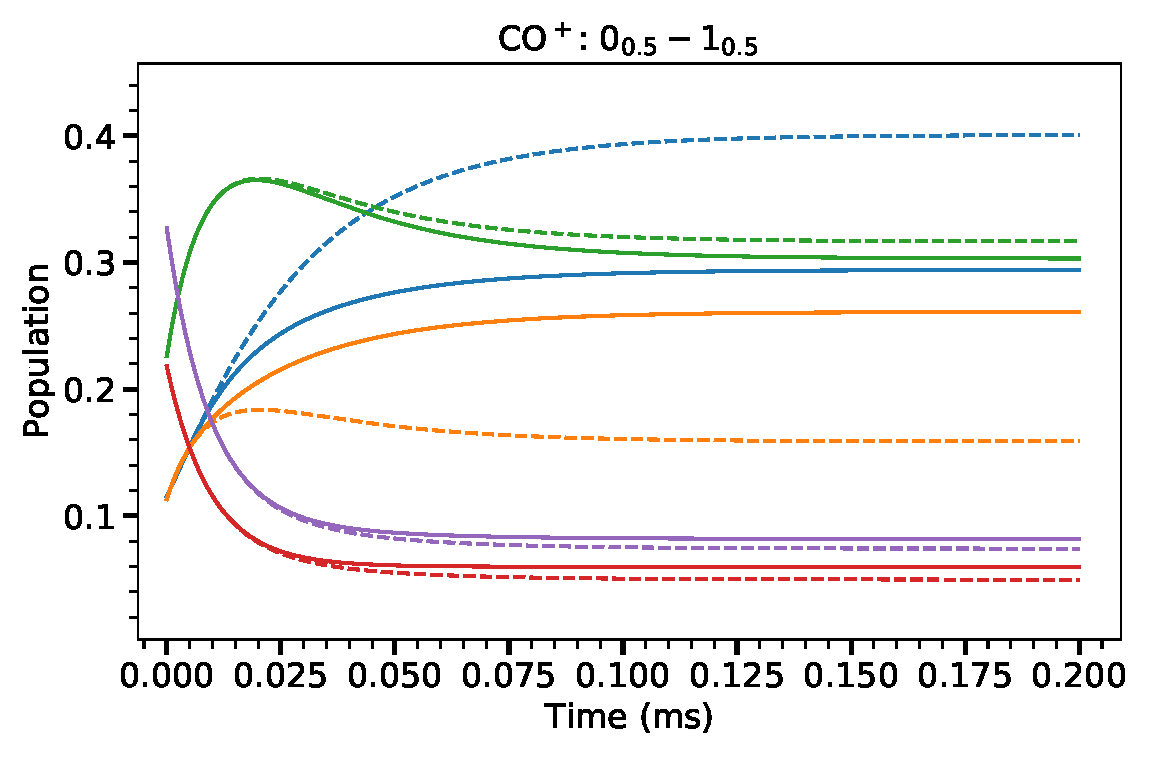
\includegraphics[width=1\textwidth]{chapters/CO+_ROSAA_paper/SI/CO^+_pop_ratio_0_0.5 - 1_0.5.pdf}
        \caption{}
    \end{subfigure}
    \hfill
    \begin{subfigure}[b]{0.49\textwidth}
        \centering
        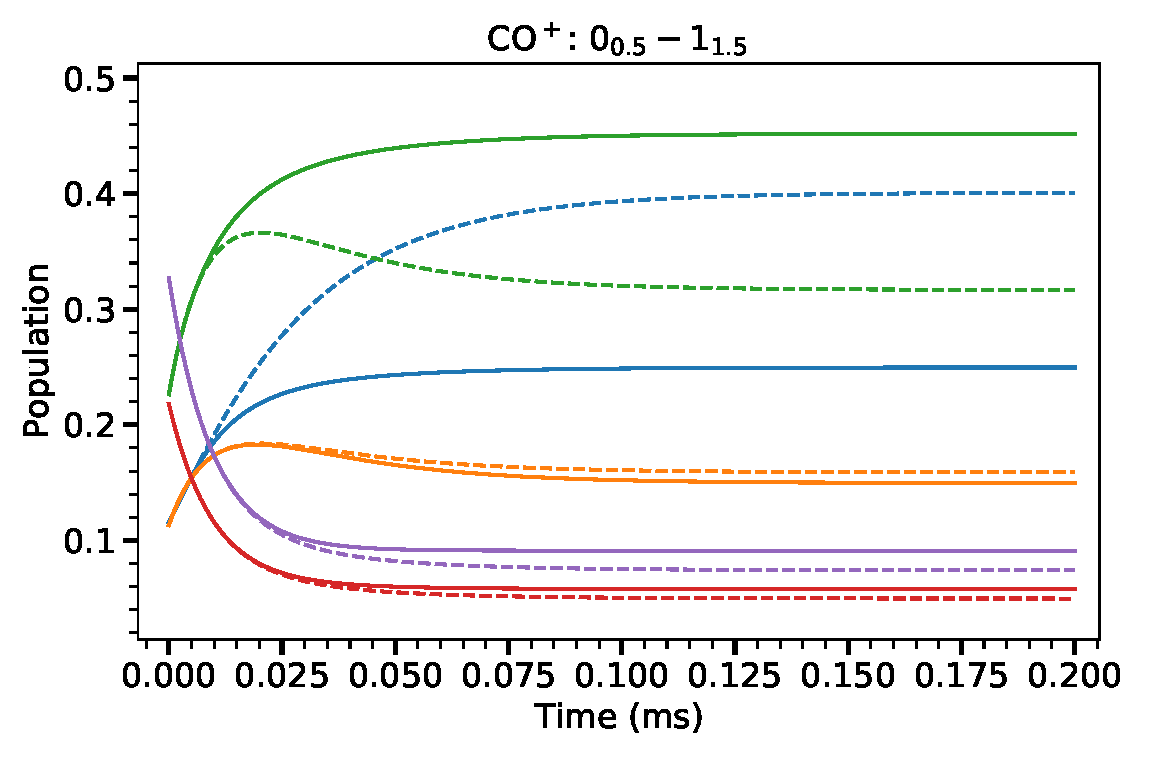
\includegraphics[width=1\textwidth]{chapters/CO+_ROSAA_paper/SI/CO^+_pop_ratio_0_0.5 - 1_1.5.pdf}
        \caption{}
    \end{subfigure}
    \hfill
    \begin{subfigure}[b]{0.49\textwidth}
        \centering
        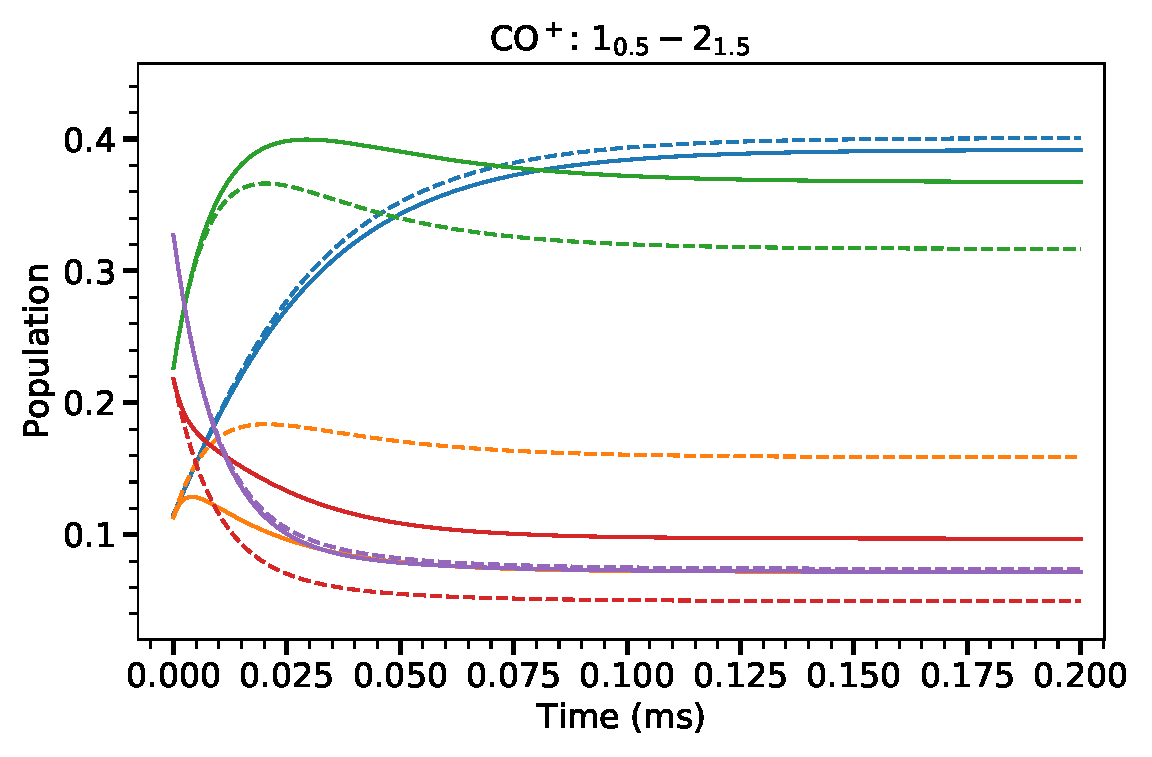
\includegraphics[width=1\textwidth]{chapters/CO+_ROSAA_paper/SI/CO^+_pop_ratio_1_0.5 - 2_1.5.pdf}
        \caption{}
    \end{subfigure}
    \hfill
    \begin{subfigure}[b]{0.49\textwidth}
        \centering
        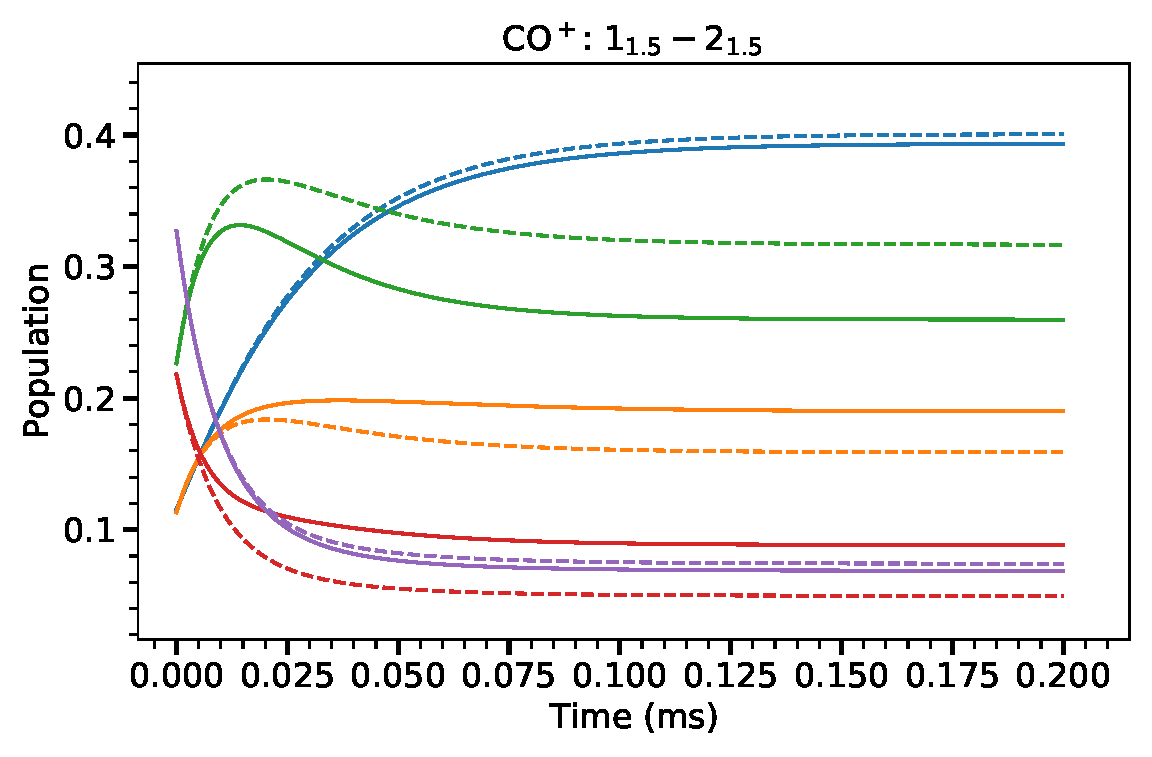
\includegraphics[width=1\textwidth]{chapters/CO+_ROSAA_paper/SI/CO^+_pop_ratio_1_1.5 - 2_1.5.pdf}
        \caption{}
    \end{subfigure}
    \caption{Numerical simulations of the rotational state population distribution of $N_J$ states with (solid line) and without (dashed line) radiation upon excitation of the transitions indicated in the title of each figure. The color code represents $N_J$ states as follows: \textcolor{blue}{\co($0_{0.5}$)}, \textcolor{orange}{\co($1_{0.5}$)}, \textcolor{green}{\co($1_{1.5}$)}, \textcolor{red}{\co($2_{1.5}$)} and  \textcolor{purple}{\co($2_{2.5}$)}. At t=0, the initial population is given by the  Boltzmann distribution at T=300 K which undergoes collisional cooling to reach collisional temperature T=$6(1)$K. The collisional rates are computed from collisional rate constants and He number density [He]$\sim 4\cdot10^{14}$~cm$^{-3}$. The radiative rates (Einstein B  coefficients for stimulated emission and absorption) are derived from Einstein A coefficients for spontaneous emission (PGOPHER simulation) with radiation power for (a) \& (b) 25$\mu W$ and (c) \& (d) 20$\mu W$.}
\end{figure}

\begin{figure}[!htb]
    \centering
    \begin{subfigure}[b]{0.49\textwidth}
        \centering
        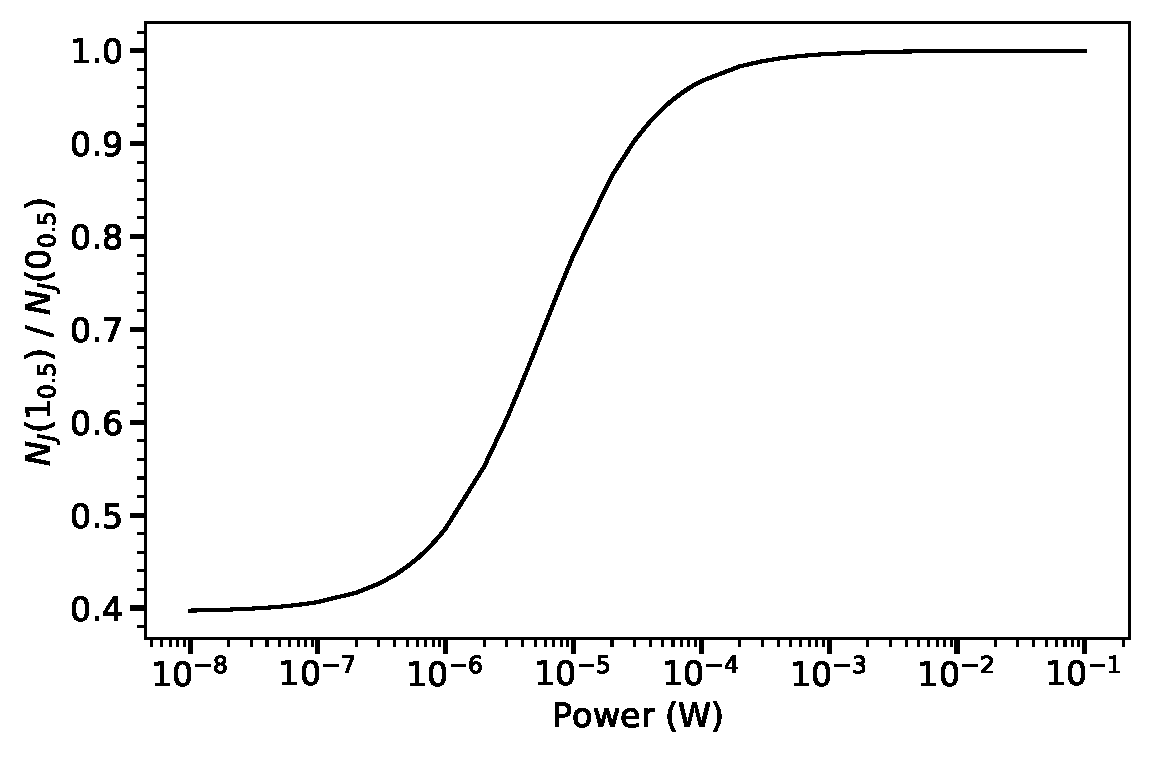
\includegraphics[width=1\textwidth]{chapters/CO+_ROSAA_paper/SI/functionOfpower_CO^+_0_0.5 - 1_0.5_4.e+14.pdf}
    \end{subfigure}
    \hfill
    \begin{subfigure}[b]{0.49\textwidth}
        \centering
        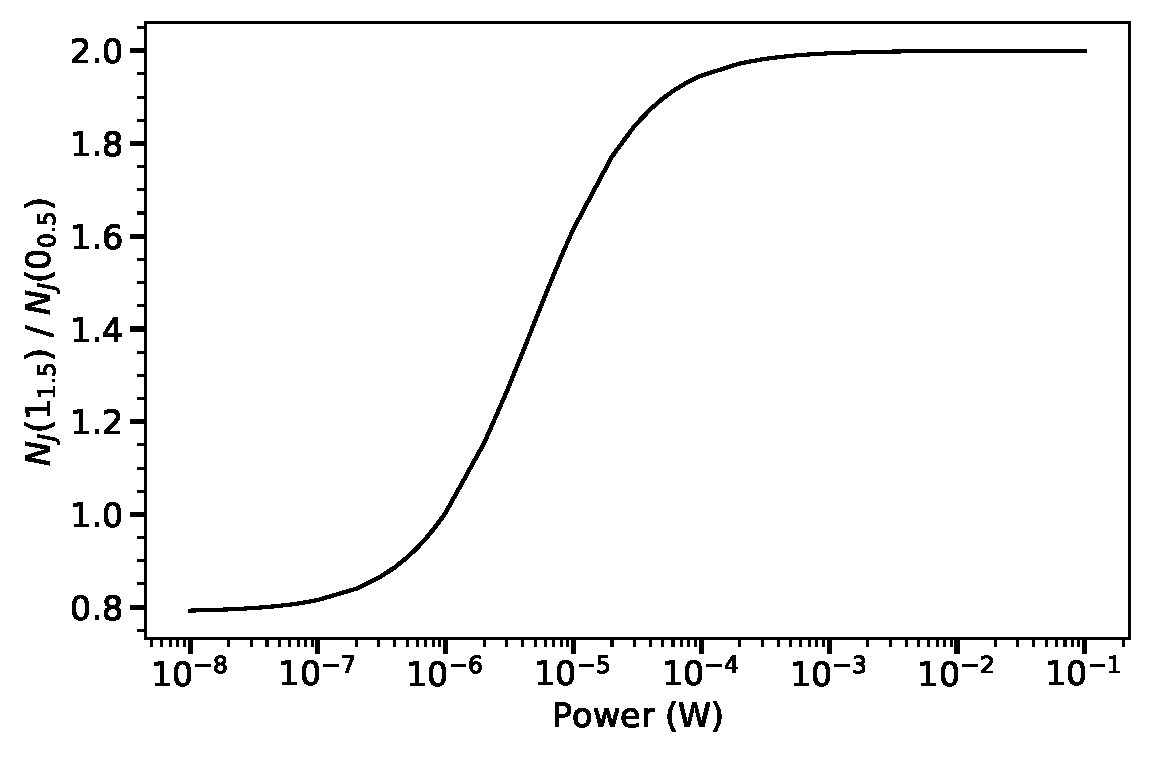
\includegraphics[width=1\textwidth]{chapters/CO+_ROSAA_paper/SI/functionOfpower_CO^+_0_0.5 - 1_1.5_4.e+14.pdf}
    \end{subfigure}
    \hfill
    \begin{subfigure}[b]{0.49\textwidth}
        \centering
        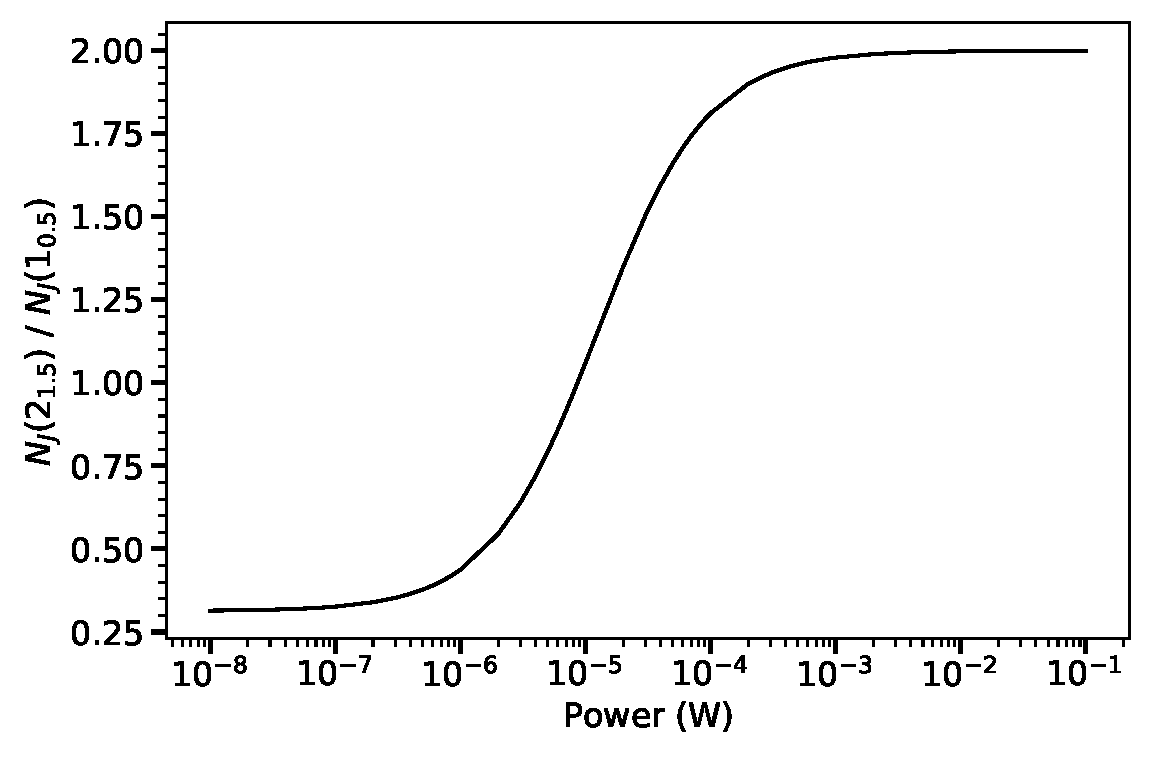
\includegraphics[width=1\textwidth]{chapters/CO+_ROSAA_paper/SI/functionOfpower_CO^+_1_0.5 - 2_1.5_4.e+14.pdf}
    \end{subfigure}
    \hfill
    \begin{subfigure}[b]{0.49\textwidth}
        \centering
        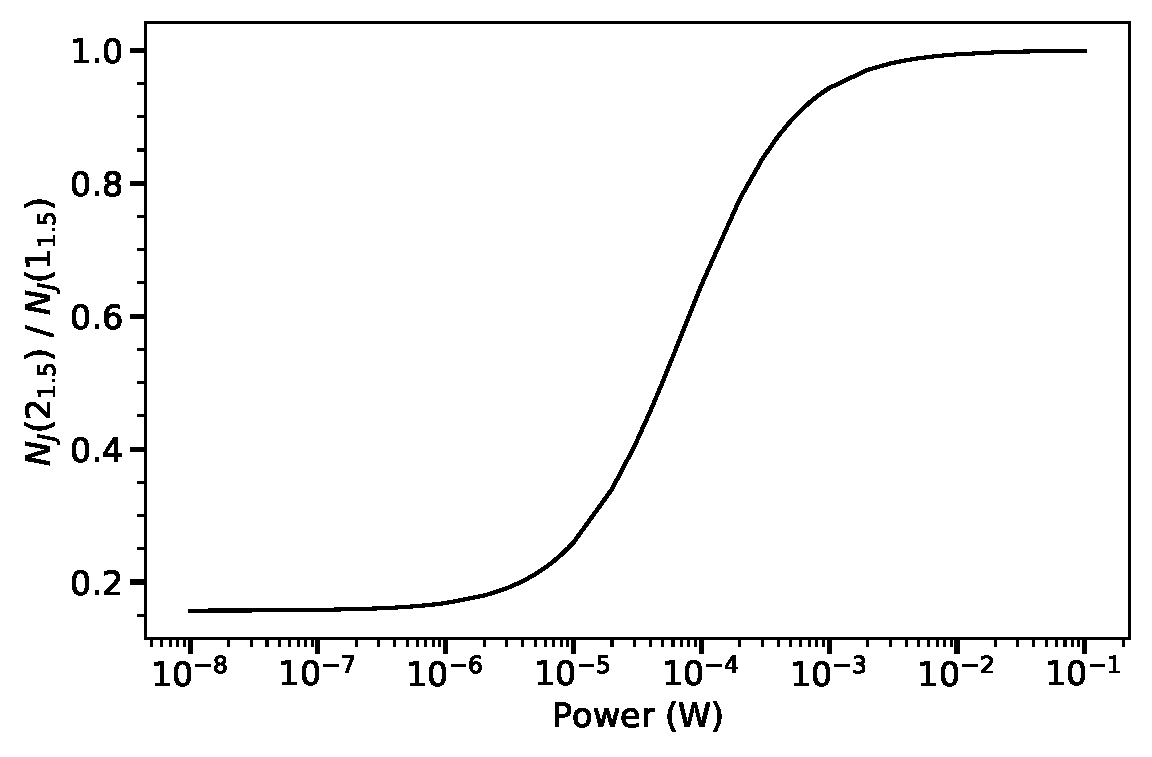
\includegraphics[width=1\textwidth]{chapters/CO+_ROSAA_paper/SI/functionOfpower_CO^+_1_1.5 - 2_1.5_4.e+14.pdf}
    \end{subfigure}
    \caption{Simulated population ratio ($N_J$: up/down) of CO$^+$ fine-structure transitions as a function of continuous excitation power on the respective transition after storing for 600ms in the trap with a constant He number density of [He]$\sim4\cdot$10$^{14}$~cm$^{-3}$.}
    \label{fig:SI:CO+:power}
\end{figure}

\begin{figure}
    \centering
    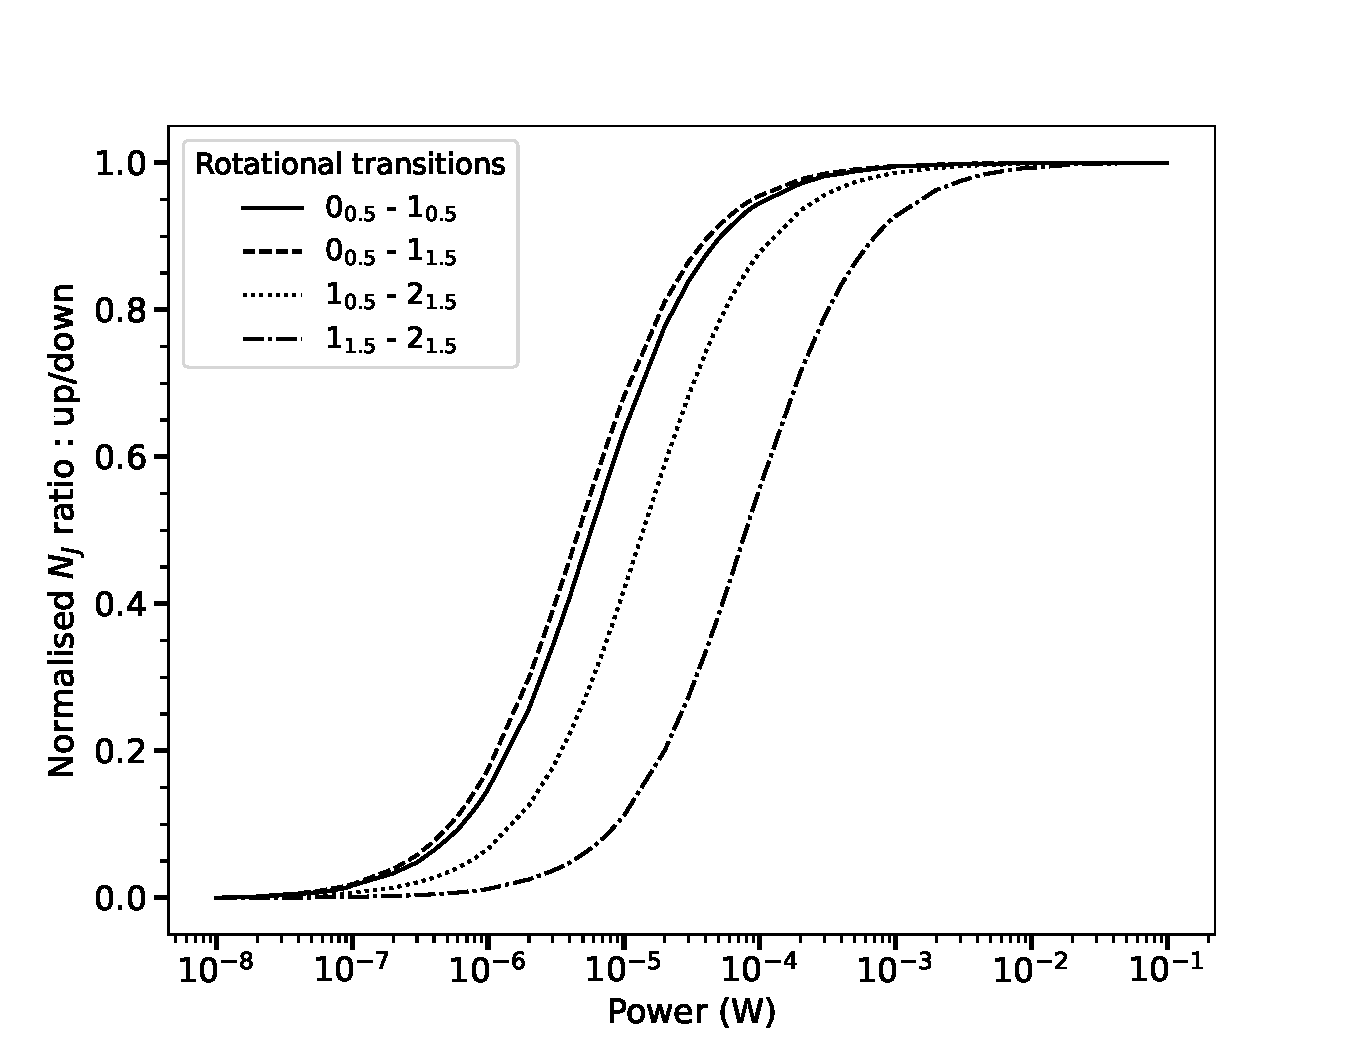
\includegraphics[width=1\textwidth]{chapters/CO+_ROSAA_paper/SI/compareTransitions.pdf}
    \caption{Comparison of the normalized simulated population ratio ($N_J$: up/down) of the respective CO$^+$ fine-structure transitions as a function of continuous excitation power on the respective transition after storing for 600ms in a trap with a constant He number density of [He]$\sim4\cdot$10$^{14}$~cm$^{-3}$. Transitions with higher transition strength reach saturation at lower excitation power.}
    \label{fig:SI:CO+:power-norm}
\end{figure}
